% adding a comment

%% This is file `elsarticle-template-1-num.tex', Copyright 2009 Elsevier Ltd
%% This file is part of the 'Elsarticle Bundle'.
%% ---------------------------------------------
%% Use the options 1p,twocolumn; 3p; 3p,twocolumn; 5p; or 5p,twocolumn for a final journal layout:
%% \documentclass[preprint,12pt]{elsarticle}
%% \documentclass[preprint,review,12pt]{elsarticle}
%% \documentclass[final,1p,times]{elsarticle}
%% \documentclass[final,1p,times,twocolumn]{elsarticle}
%% \documentclass[final,3p,times]{elsarticle}
%% \documentclass[final,5p,times]{elsarticle}
%% \documentclass[final,5p,times,twocolumn]{elsarticle}

\documentclass[preprint, 5p, times, twocolumn]{elsarticle}
\usepackage{graphicx}
\usepackage{amssymb}
\usepackage{amsmath}
\usepackage{lineno}
\usepackage{dblfloatfix}
\usepackage{setspace}
\usepackage{xr}
\externaldocument{../PhaseIIPaper/supdocs/supdocs}
%\usepackage[citecolor=blue]{hyperref}
\usepackage{xcolor}
\usepackage{enumitem}

\bibliographystyle{model5-names.bst}
\biboptions{authoryear, comma}
\journal{Agricultural and Forest Meteorology}
\doublespacing

\begin{document}
\begin{frontmatter}

\title{The GGCMI Phase II experiment: simulating and emulating global crop yield responses to changes in carbon dioxide, temperature, water, and nitrogen levels}

\author[1,2]{James Franke\corref{cor1}}
\author[2,3]{Joshua Elliott}
\author[4]{Christoph M\"{u}ller}
\author[5]{Alexander Ruane}
\author[6]{Abigail Snyder}
\author[3,2,4,5]{Jonas J\"{a}germeyr}
\author[7,8]{Juraj Balkovic}
\author[9,10]{Philippe Ciais}
\author[11]{Marie Dury}
\author[12]{Pete Falloon}
\author[7]{Christian Folberth}
\author[11]{Louis Fran{\c{c}}ois}
\author[13]{Tobias Hank}
\author[14]{Munir Hoffmann}
\author[15,16]{Cesar Izaurralde}
\author[11]{Ingrid Jacquemin}
\author[15]{Curtis Jones}
\author[7]{Nikolay Khabarov}
\author[14]{Marian Koch}
\author[2, 17]{Michelle Li}
\author[18,9]{Wenfeng Liu}
\author[19]{Stefan Olin}
\author[5,20]{Meridel Phillips}
\author[21,22]{Thomas Pugh}
\author[15]{Ashwan Reddy}
\author[9,10]{Xuhui Wang}
\author[12]{Karina Williams}
\author[13]{Florian Zabel}
\author[1,2]{Elisabeth Moyer}
%%%%%%%%%%%%%%%%%%%%%%%%%%%%%%

\address[1]{Department of the Geophysical Sciences, University of Chicago, Chicago, IL, USA}
\address[2]{Center for Robust Decision-making on Climate and Energy Policy (RDCEP), University of Chicago, Chicago, IL, USA}
\address[3]{Department of Computer Science, University of Chicago, Chicago, IL, USA}
\address[4]{Potsdam Institute for Climate Impact Research, Leibniz Association (Member), Potsdam, Germany}
\address[5]{NASA Goddard Institute for Space Studies, New York, NY, United States}
\address[6]{Joint Global Change Research Institute, Pacific Northwest National Laboratory, College Park, MD, USA}
\address[7]{Ecosystem Services and Management Program, International Institute for Applied Systems Analysis, Laxenburg, Austria}
\address[8]{Department of Soil Science, Faculty of Natural Sciences, Comenius University in Bratislava, Bratislava, Slovak Republic}
\address[9]{Laboratoire des Sciences du Climat et de l'Environnement,
CEA-CNRS-UVSQ, 91191 Gif-sur-Yvette, France}
\address[10]{Sino-French Institute of Earth System Sciences, College of Urban and
Environmental Sciences, Peking University, Beijing, China}
\address[11]{Unit{\'{e}} de Mod{\'{e}}lisation du Climat et des Cycles Biog\'eochimiques, UR SPHERES, Institut d'Astrophysique et de G\'eophysique, University of Li\`ege, Belgium}
\address[12]{Met Office Hadley Centre, Exeter, United Kingdom}
\address[13]{Department of Geography, Ludwig-Maximilians-Universit\"{a}t, Munich, Germany}
\address[14]{Georg-August-University G\"{o}ttingen, Tropical Plant Production and Agricultural Systems Modelling, G\"{o}ttingen, Germany}
\address[15]{Department of Geographical Sciences, University of Maryland, College Park, MD, USA}
\address[16]{Texas Agrilife Research and Extension, Texas A\&M University, Temple, TX, USA}
\address[17]{Department of Statistics, University of Chicago, Chicago, IL, USA}
\address[18]{EAWAG, Swiss Federal Institute of Aquatic Science and Technology, D\"{u}bendorf, Switzerland}
\address[19]{Department of Physical Geography and Ecosystem Science, Lund University, Lund, Sweden}
\address[20]{Earth Institute Center for Climate Systems Research, Columbia University, New York, NY, USA}
\address[21]{Karlsruhe Institute of Technology, IMK-IFU, 82467 Garmisch-Partenkirchen, Germany.}
\address[22]{School of Geography, Earth and Environmental Science, University of Birmingham, Birmingham, UK.}

\cortext[cor1]{Corresponding author at: 4734 S Ellis, Chicago, IL 60637, United States. email: jfranke@uchicago.edu}

\begin{abstract}
{\color{blue} Concerns about food security under climate change have motivated efforts to better understand the future changes in yields by using detailed process-based models in agronomic sciences.
Process-based models differ on many details affecting yields and considerable uncertainty remains in future yield projections.
Phase II of the Global Gridded Crop Model Intercomparison (GGCMI), an activity of the Agricultural Model Intercomparison and Improvement Project (AgMIP), consists of a large simulation set with perturbations in atmospheric CO$_2$ concentrations, temperature, precipitation, and applied nitrogen inputs and constitutes a data-rich basis of projected yield changes across twelve models and five crops (maize, soy, rice, spring wheat, and winter wheat) using global gridded simulations.
In this paper we present the simulation output database from Phase II of the GGCMI effort, a targeted experiment aimed at understanding the sensitivity to and interaction between multiple climate variables (as well as management) on yields, and illustrate some initial summary results from the model intercomparison project.
We also present the construction of a simple ``emulator’’ or statistical representation of the simulated 30-year mean climatological output in each location for each crop and model.
The emulator captures the response of the process-based models in a lightweight, computationally tractable form that facilitates model comparison as well as potential applications in subsequent modeling efforts such as integrated assessment.}

%Results of these models are often used to inform subsequent model-based analyses in agricultural economics and integrated assessment, but the computational requirements of process-based models sometimes hamper the ability to utilize these models in existing impact assessment frameworks at high resolutions globally. 
%Models robustly produce yield responses that are nonlinear and sensitive to interactions across the input variables. 
%Results illustrate the utility of model emulation for climate impacts studies.
%Fundamental feedbacks between economic decision making and crop performance (e.g.\ management for intensification) is often ignored, as better integration of the different model types is hampered by the computational requirements of detailed deterministic process-based crop models and optimization-based economic modeling frameworks. 
% STEFAN: Why? Differences among models is not an aim, is an outcome from the fact that much is still unknown regarding first principles.
%Results show considerable spatial heterogeneity in sensitivity to input variables, confirming the need for a global study, as well as differences across models.
% STEFAN: Have other studies confirmed that? Otherwise it's not an aim in itself to have that as an outcpme of this study.
\end{abstract}

\begin{keyword}
climate change \sep food security \sep model emulation \sep AgMIP \sep crop model
\end{keyword}
\end{frontmatter}

\modulolinenumbers[1]
\linenumbers
%%%%%%%%%%%%%%%%%%%%%%%%%%%%%%%%%%%%%%%%%%%%%%%%%%%%%%%%%%%%%%%%%%%%%
\section{Introduction}
\label{S:1}

Understanding crop yield response to a changing climate is critically important, especially as the global food production system will face pressure from increased demand over the next century. Climate-related reductions in supply could therefore have severe socioeconomic consequences. Multiple studies using different crop or climate models concur in predicting sharp yield reductions on currently cultivated cropland under {business-as-usual} climate scenarios, although their yield projections show considerable spread \citep[e.g.][and references therein]{porter2014, Rosenzweig2014, Schauberger2017}. 
%These differences are unsurprising because 
Modeling crop responses continues to be challenging, as crop 
%responses in models can be complex, with crop 
growth is a function of complex interactions between climate inputs and management practices. 
% XX closing sentence saying "therefore we need..."?

Computational models have been used to project crop yields since the 1950's, beginning with statistical models  that attempt to capture the relationship between input factors and resultant yields \citep[e.g.][]{Heady57, Heady61}. These statistical models were typically developed on a small scale for locations with extensive histories of yield data. The emergence of electronic computers allowed development of numerical models that simulate the process of photosynthesis and the biology and phenology of individual crops (first proposed by \citet{wit58} and \cite{Duncan67} and attempted by \citet{Duncan72}; for a history of crop model development see \citet{Rosenzweig2014}). A half-century of improvement in both models and computing resources means that researchers can now run crop simulations for many years at high spatial resolution on the global scale. 

Both types of models continue to be used, and comparative studies have concluded that when done carefully, both approaches can provide similar yield estimates \citep[e.g.][]{Lobell2010, Moore2017, Roberts2017, zhao2017}. Models tend to agree broadly in major response patterns, including a reasonable representation of the spatial pattern in historical yields of major crops \citep[e.g.][]{Elliott2015, muller_global_2017} and projections of decreases in yield under future climate scenarios.

Process-based models do continue to struggle with some important details, including reproducing historical year-to-year variability \citep[e.g.][]{muller_global_2017}, reproducing historical yields when driven by reanalysis weather \citep[e.g.][]{Glotter14}, and low sensitivity to extreme events \citep[e.g.][]{Glotter15}. These issues are driven in part by the diversity of new cultivars and genetic variants, which outstrips the ability of academic modeling groups to capture them \citep[e.g.][]{JONES2017b}. Models also do not simulate many additional factors affecting production, including pests, diseases, and weeds. For these reasons, individual studies must generally re-calibrate models to ensure that short-term predictions reflect current cultivar mixes, and long-term projections retain considerable uncertainty \citep{WOLF2002217, JAGTAP200273, Iizumi2010, ANGULO201332, Asseng2013, Asseng2015}. Inter-model discrepancies can also be high in areas not yet cultivated \citep[e.g.][]{Challinor2014, WHITE2011357}. Finally, process-based models present additional difficulties for high-resolution global studies because of their complexity and computational requirements. For economic impacts assessments, it is often impossible to integrate a set of process-based crop models directly into an integrated assessment model to estimate the potential cost of climate change to the agricultural sector.

Nevertheless, process-based models are necessary for understanding the global future yield impacts of climate change for many reasons. First, cultivation may shift to new areas, where no yield data are currently available and therefore statistical models cannot apply. Yield data are also often limited in the developing world, where future climate impacts may be the most critical. Finally, only process-based models can capture the growth response to novel conditions and practices that are not represented in historical data \citep[e.g.][]{pugh_climate_2016, Roberts2017}. These novel changes can include the direct fertilization effect of elevated CO$_2$, or changes in management practices that may ameliorate climate-induced damages.

Interest has been rising in statistical emulation, which allows combining advantageous features of both statistical and process-based models. The approach involves constructing a statistical representation or ``surrogate model'' of complicated numerical simulations by using simulation output as the training data for a statistical model \citep[e.g.][]{OHAGAN2006, OHAGAN2010}. Emulation is particularly useful in cases where simulations are complex and output data volumes are large,  and  has been used in a variety of fields, including hydrology \citep[e.g.][]{Razavi2012}, engineering \citep[e.g.][]{STORLIE2009}, environmental sciences \citep[e.g.][]{RATTO2012}, and climate \citep[e.g.][]{Castruccio14, Holden2014}. For agricultural impacts studies, emulation of process-based models allows capturing key relationships between input variables in a lightweight, flexible form that is compatible with economic studies. 

In the past decade, multiple studies have developed emulators of process-based crop simulations. Early studies proposing or describing potential crop yield emulators include \citet{Howden2005, raisen2006, Lobell2010}, and \citet{Ferrise2011}, who used a machine learning approach to predict Mediterannean wheat yields. Studies developing single-model emulators include  \citet{Holzkamper2012} for the CropSyst model, \citet{RUANE2013a} for the CERES wheat model, and \citet{Oyebamiji15} for the LPJmL model (for multiple crops, using multiple scenarios as a training set). More recently, emulators have begun to be used in the context of multi-model intercomparisons, with \citet{BLANC2015, BLANC2017, Ostberg2018} and \citet{Mistry2017} using them to analyze the five crop models of the Inter-Sectoral Impacts Model Intercomparison Project (ISIMIP) \citep{Warszawski3228}, which simulated yields for maize, soy, wheat, and rice. Choices differ: \citet{BLANC2015} and \citet{BLANC2017} base their emulation on historical simulations and a single future climate/emissions scenario (RCP8.5), and use local weather variables and yields in their regression but then aggregate across broad regions; \citet{Ostberg2018} consider multiple future climate scenarios, using global mean temperature change (and CO$_2$) as regressors but then pattern-scale to emulate local yields; while \citet{Mistry2017} attempt to compare emulated historical yearly yields to observed historical yields, using local weather data and a historical crop simulation. These efforts do share important common features: all emulate annual crop yields across the entire scenario or scenarios, and when future scenarios are considered, they are non-stationary, i.e.\ their input climate parameters evolve over time.

An alternative approach is to construct a training set of multiple stationary scenarios in which parameters are systematically varied. Such a ``parameter sweep'' offers several advantages for emulation over scenarios in which climate evolves over time.  First, it allows separating the effects of different variables that impact yields but that are highly correlated in realistic future scenarios (e.g.\ CO$_2$ and temperature). Second, it allows making a distinction between year-over-year yield variations and climatological changes, which may involve different responses to the particular climate regressors used \citep[e.g.][]{Ruane2016}. For example, if year-over-year yield variations are driven predominantly by variations in the distribution of temperatures throughout the growing season, and long-term climate changes are driven predominantly by shifts in means, then regressing on the mean growing season temperature will produce different yield responses at annual vs.\ climatological timescales.  

Systematic parameter sweeps have begun to be used in crop model evaluation and emulation, with
early efforts in 2015 \citep{Markowski2015, Pirttioja2015}, and several recent studies in 2018 \citep{FRONZEK20182, Snyder2018, RUIZRAMOS2018}. All three studies sample multiple perturbations to temperature and precipitation (with \citet{Snyder2018} and \citet{RUIZRAMOS2018} adding CO$_2$ as well), in 132, 99 and 220 different combinations, respectively, and take advantage of the structured training set to construct emulators (aka response surfaces in this context) of climatological mean yields, omitting year-over-year variations. The main limitation in these studies is geographic extent, with each study focusing on a limited number of sites. \citet{FRONZEK20182} and \citet{RUIZRAMOS2018} simulate only wheat (over several models) and \citet{Snyder2018} analyzes analyzes four crops (maize, wheat, rice, soy) based on site-specific crop model sensitivity tests from the C3MP project \citep{mcdermid2015}.

%Both studies are limited in other aspects, however: both simulate only a handful of individual sites, and \citet{FRONZEK20182} simulates only wheat (over several models), while \citet{Snyder2018} analyzes four crops but with a single model (GCAM). 
%  t also removes the correlation between the key variables driving yields which may prove difficult to disentangle in RCP climate model runs and it provides fully stationary simulations. %A parameter sweep across the major drivers 

\begin{figure}[!ht]
\centering
   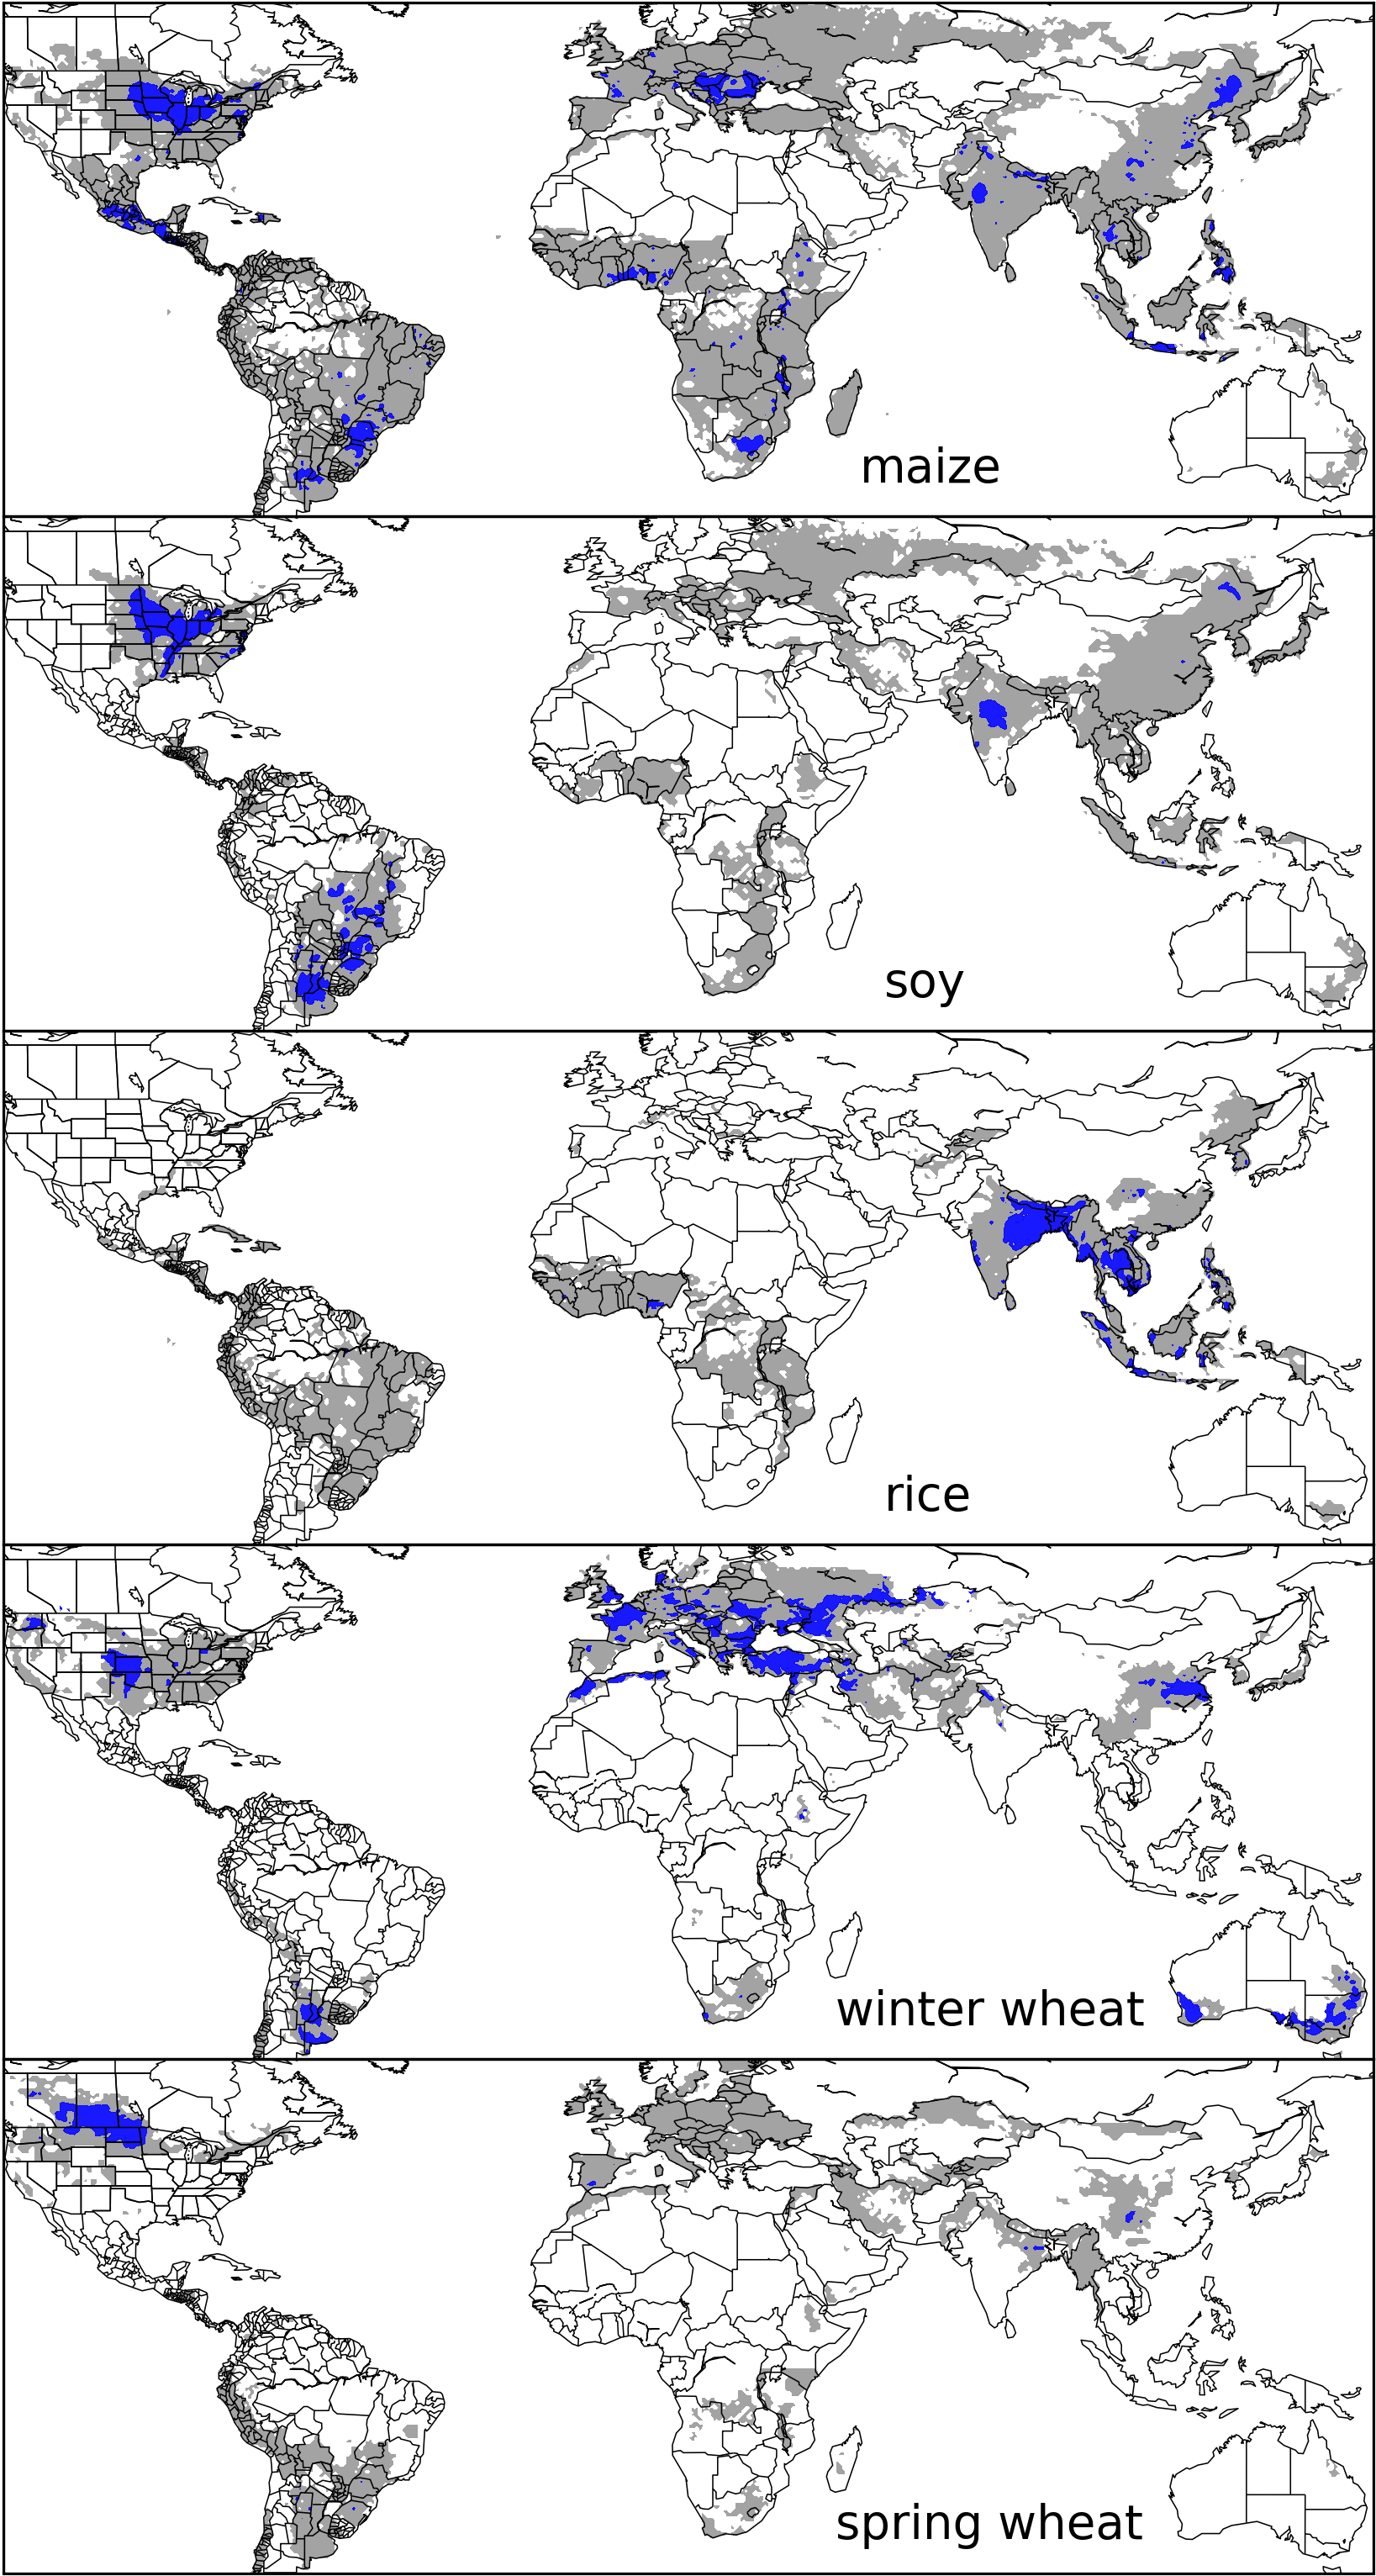
\includegraphics[width=0.95\linewidth]{figures/croparea.png}
   \caption{Presently cultivated area for rain-fed crops. Blue indicates grid cells with more that 20,000 hectares ($\sim$10\% of the equatorial grid cells) of crop cultivated. Gray contour shows area with more that 10 hectares cultivated. Cultivated areas for maize, rice, and soy are taken from the MIRCA2000 (``monthly irrigated and rain-fed crop areas around the year 2000'') dataset \citep{Portmann2010}. Areas for winter and spring wheat areas are adapted from MIRCA2000 data and sorted by growing season. For analogous figure of irrigated crops, see Figure \ref{fig:irrarea}.}
   \label{fig:crop_area}
\end{figure}

\begin{table*}[!hb]
    \small \centering
    \begin{tabular}[0.75\linewidth]{lccc} 
        \hline \vspace{1mm}
        \textbf{Input variable} & \textbf{Abbr.} & \textbf{Tested range} & \textbf{Unit}\\ \hline \hline \vspace{1mm}
        {CO$_2$}& {C} & {360, 510, 660, 810} & {ppm}\\ \hline \vspace{1mm}
        {Temperature}& {T} & {-1, 0, 1, 2, 3, 4, 5*, 6} & {$^{\circ}$C}\\ \hline \vspace{1mm}
        {Precipitation}& {W} & {-50, -30, -20, -10, 0, 10, 20, 30, (and W$_{inf}$)} & {\%}\\ \hline \vspace{1mm}
        {Applied nitrogen}& {N} & {10, 60, 200} & {kg ha$^{-1}$}\\ \hline
    \end{tabular}\\
    \parbox{11cm}{\caption{GGCMI Phase II input variable test levels. Temperature and precipitation values indicate the perturbations from the historical, climatology. * Only simulated by one model. W-percentage does not apply to the irrigated (W$_{inf}$) simulations, which are all simulated at the maximum benficial levels of water.}}
    \label{table:inputs}
\end{table*}

In this paper we describe a new comprehensive dataset designed to expand the parameter sweep approach still further. The Global Gridded Crop Model Intercomparison (GGCMI) Phase II experiment involves running a suite of process-based crop models across historical conditions perturbed by a set of discrete steps in different input parameters, including an applied nitrogen dimension. The experimental protocol involves over 700 different parameter combinations for each model and crop, with simulations providing near-global coverage at a half degree spatial resolution. The experiment was conducted as part of the Agricultural Model Intercomparison and Improvement Project (AgMIP) \citep{ROSENZWEIG2013, Rosenzweig2014}, an international effort conducted under a framework similar to the Climate Model Intercomparison Project (CMIP) \citep{Taylor2012, Eyring2016}. The GGCMI protocol builds on the AgMIP Coordinated Climate-Crop Modeling Project (C3MP) \citep{ruane2014, mcdermid2015} and will contribute to the AgMIP Coordinated Global and Regional Assessments (CGRA) \citep{ruane2018, rosenzweig2018}. GGCMI Phase II is designed to allow addressing goals such as understanding where highest-yield regions may shift under climate change; exploring future adaptive management strategies; understanding how interacting input drivers affect crop yield; quantifying uncertainties across models and major drivers; and testing strategies for producing lightweight emulators of process-based models. In this paper, we describe the GGCMI Phase II experiments, present initial results, and demonstrate that it is tractable to emulation.

\section{Simulation -- Methods}
\label{S:2}
GGCMI Phase II is the continuation of a multi-model comparison exercise begun in 2014. The initial Phase I compared harmonized yields of 21 models for 19 crops over a 31-year historical (1980-2010) scenario with a primary goal of model evaluation \citep{Elliott2015, muller_global_2017}. Phase II compares simulations of 12 models for 5 crops (maize, rice, soybean, spring wheat, and winter wheat) over the same historical time series (1980-2010) used in Phase I, but with individual climate or management inputs adjusted from their historical values. The reduced set of crops includes the three major global cereals and the major legume and accounts for over 50\% of human calories (in 2016, nearly 3.5 billion tons or 32\% of total global crop production by weight \citep{FAOSTAT}. 

\begin{table*}[!t]
    \small \centering
    \begin{tabular}{p{7cm} | p{1cm} p{1cm} p{1cm} p{1cm} p{1cm} p{1cm} | p{1.5cm}}
        \hline
        \textbf{Model (Key Citations)} & \textbf{Maize} & \textbf{Soy} & \textbf{Rice} & \textbf{Winter Wheat} & \textbf{Spring Wheat} & \textbf{N Dim.} & \textbf{Simulations per Crop}\\ \hline \hline
        {\textbf{APSIM-UGOE},    \citet{KEATING2003267, HOLZWORTH2014327}} & {X} & {X} & {X} & {--} & {X} & {Yes} & {37}\\ \hline
        {\textbf{CARAIB},        \citet{Dury2011, Pirttioja2015}} & {X} & {X} & {X} & {X} & {X} & {No} & {224}\\ \hline
        {\textbf{EPIC-IIASA},    \citet{BALKOVIC2014}} & {X} & {X} & {X} & {X} & {X} & {Yes} & {35}\\  \hline
        {\textbf{EPIC-TAMU},     \citet{Izaurralde06}} & {X} & {X} & {X} & {X} & {X} & {Yes} & {672}\\ \hline
        {\textbf{JULES*},        \citet{Osborne2015, Williams2015, Williams2017}} & {X} & {X} & {X} & {--} & {X} & {No} & {224}\\ \hline
        {\textbf{GEPIC},         \citet{LIU2007478, FOLBERTH201221}} & {X} & {X} & {X} & {X} & {X} & {Yes} & {384}\\ \hline
        {\textbf{LPJ-GUESS},     \citet{Lindeskog2013, Olin2015}} & {X} & {--} & {--} & {X} & {X} & {Yes} & {672}\\  \hline
        {\textbf{LPJmL},         \citet{von_Bloh_implementing_2018}} & {X} & {X} & {X} & {X} & {X} & {Yes} & {672}\\ \hline
        {\textbf{ORCHIDEE-crop}, \citet{Valade2013}} & {X} & {--} & {X} & {--} & {X} & {Yes} & {33}\\ \hline
        {\textbf{pDSSAT},        \citet{Elliott2014b, JONES2003235}} & {X} & {X} & {X} & {X} & {X} & {Yes} & {672}\\ \hline
        {\textbf{PEPIC},         \citet{LIU2016164, LIU2016}} & {X} & {X} & {X} & {X} & {X} & {Yes} & {130}\\ \hline
        {\textbf{PROMET*\dag},   \citet{MAUSER2009362, Hank2015, MAUSER2015}} & {X} & {X} & {X} & {X} & {X} & {Yes\dag} & {239}\\ \hline \hline
        {Totals} & {12} & {10} & {11} & {9} & {12} & {--} & {3993 (maize)}\\
        \hline
    \end{tabular}
 \caption{Models included in GGCMI Phase II and the number of C, T, W, and N simulations that each performs for rain-fed crops (``Sims per Crop''), with 672 as the maximum. ``N-Dim.'' indicates whether the simulations include varying nitrogen levels. Two models provide only one nitrogen level, and \dag PROMET provides only two of the three nitrogen levels (and so is not emulated across the nitrogen dimension). All models provide the same set of simulations across all modeled crops, but some omit individual crops. (For example, APSIM does not simulate winter wheat.) Irrigated simulations are provided at the level of the other covariates for each model, i.e.\ an additional 84 simulations for fully-sampled models. Simulations are nearly global but their geographic extent can vary, even for different crops in an individual model, since some simulations omit regions far outside the currently cultivated area. In most cases, historical daily climate inputs are taken from the 0.5 degree NASA AgMERRA daily gridded re-analysis product specifically designed for agricultural modeling, with satellite-corrected precipitation \citep{Ruane2015}, but two models (marked with *) require sub-daily input data and use alternative sources. See \citet{Elliott2015} for additional details.
 } 
\label{table:models}
\end{table*}

The guiding scientific rationale of GGCMI Phase II is to provide a comprehensive, systematic evaluation of the response of process-based crop models to different values for carbon dioxide, temperature, water, and applied nitrogen (collectively known as ``CTWN'').
The dataset is designed to allow researchers to:
\begin{itemize}[noitemsep]
    \item Enhance understanding of how models work by characterizing their sensitivity to input climate and nitrogen drivers.
    \item Study the interactions between climate variables and nitrogen inputs in driving modeled yield impacts. 
    \item Explore differences in crop response to warming across the Earth's climate regions.
    \item Provide a dataset that allows statistical emulation of crop model responses for downstream modelers.
    \item Illustrate differences in potential adaptation via growing season changes. 
\end{itemize}

\vspace{-0.05in}
The experimental protocol consists of 9 levels for precipitation perturbations, 7 for temperature, 4 for CO$_2$, and 3 for applied nitrogen, for a total of 672 simulations for rain-fed agriculture and an additional 84 for irrigated (Table \ref{table:inputs}). For irrigated simulations, soil water is held at either field capacity or, for those models that include water-log damage, at maximum beneficial level. Temperature perturbations are applied as absolute offsets from the daily mean, minimum, and maximum temperature time series for each grid cell used as inputs. Precipitation perturbations are applied as fractional changes at the grid cell level, and carbon dioxide and nitrogen levels are specified as discrete values applied uniformly over all grid cells. Note that CO$_2$ changes are applied independently of changes in climate variables, so that higher CO$_2$ is not associated with higher temperatures. An additional, identical set of scenarios (at the same C, T, W, and N levels) not shown or analyzed here simulate adaptive agronomy under climate change by varying the growing season for crop production. The resulting GGCMI Phase II dataset captures a distribution of crop responses over the potential space of future climate conditions.

The 12 models included in GGCMI Phase II are all mechanistic process-based crop models that are widely used in impacts assessments (Table \ref{table:models}). Although some models share a common base (e.g.\ the LPJ family or the EPIC family of models), they have subsequently developed independently. (For more details on model genealogy, see Figure S1 in \citet{Rosenzweig2014}.) Differences in model structure mean that several key factors are not standardized across the experiment, including secondary soil nutrients, carry-over effects across growing years including residue management and soil moisture, and the extent of simulated area for different crops. 
Growing seasons are standardized across models (with assumptions based on \citet{Sacks2010} and \citet{Portmann2008, Portmann2010}), but vary by crop and by location on the globe.
For example, maize is sown in March in Spain, in July in Indonesia, and in December in Namibia. All stresses are disabled other than factors related to nitrogen, temperature, and water (e.g.\ alkalinity and salinity). No additional nitrogen inputs, such as atmospheric deposition, are considered, but some model treatment of soil organic matter may allow additional nitrogen release through mineralization. See \citet{Rosenzweig2014}, \citet{Elliott2015} and \citet{muller_global_2017} for further details on models and underlying assumptions.

\begin{figure*}[!!hb]
\centering
   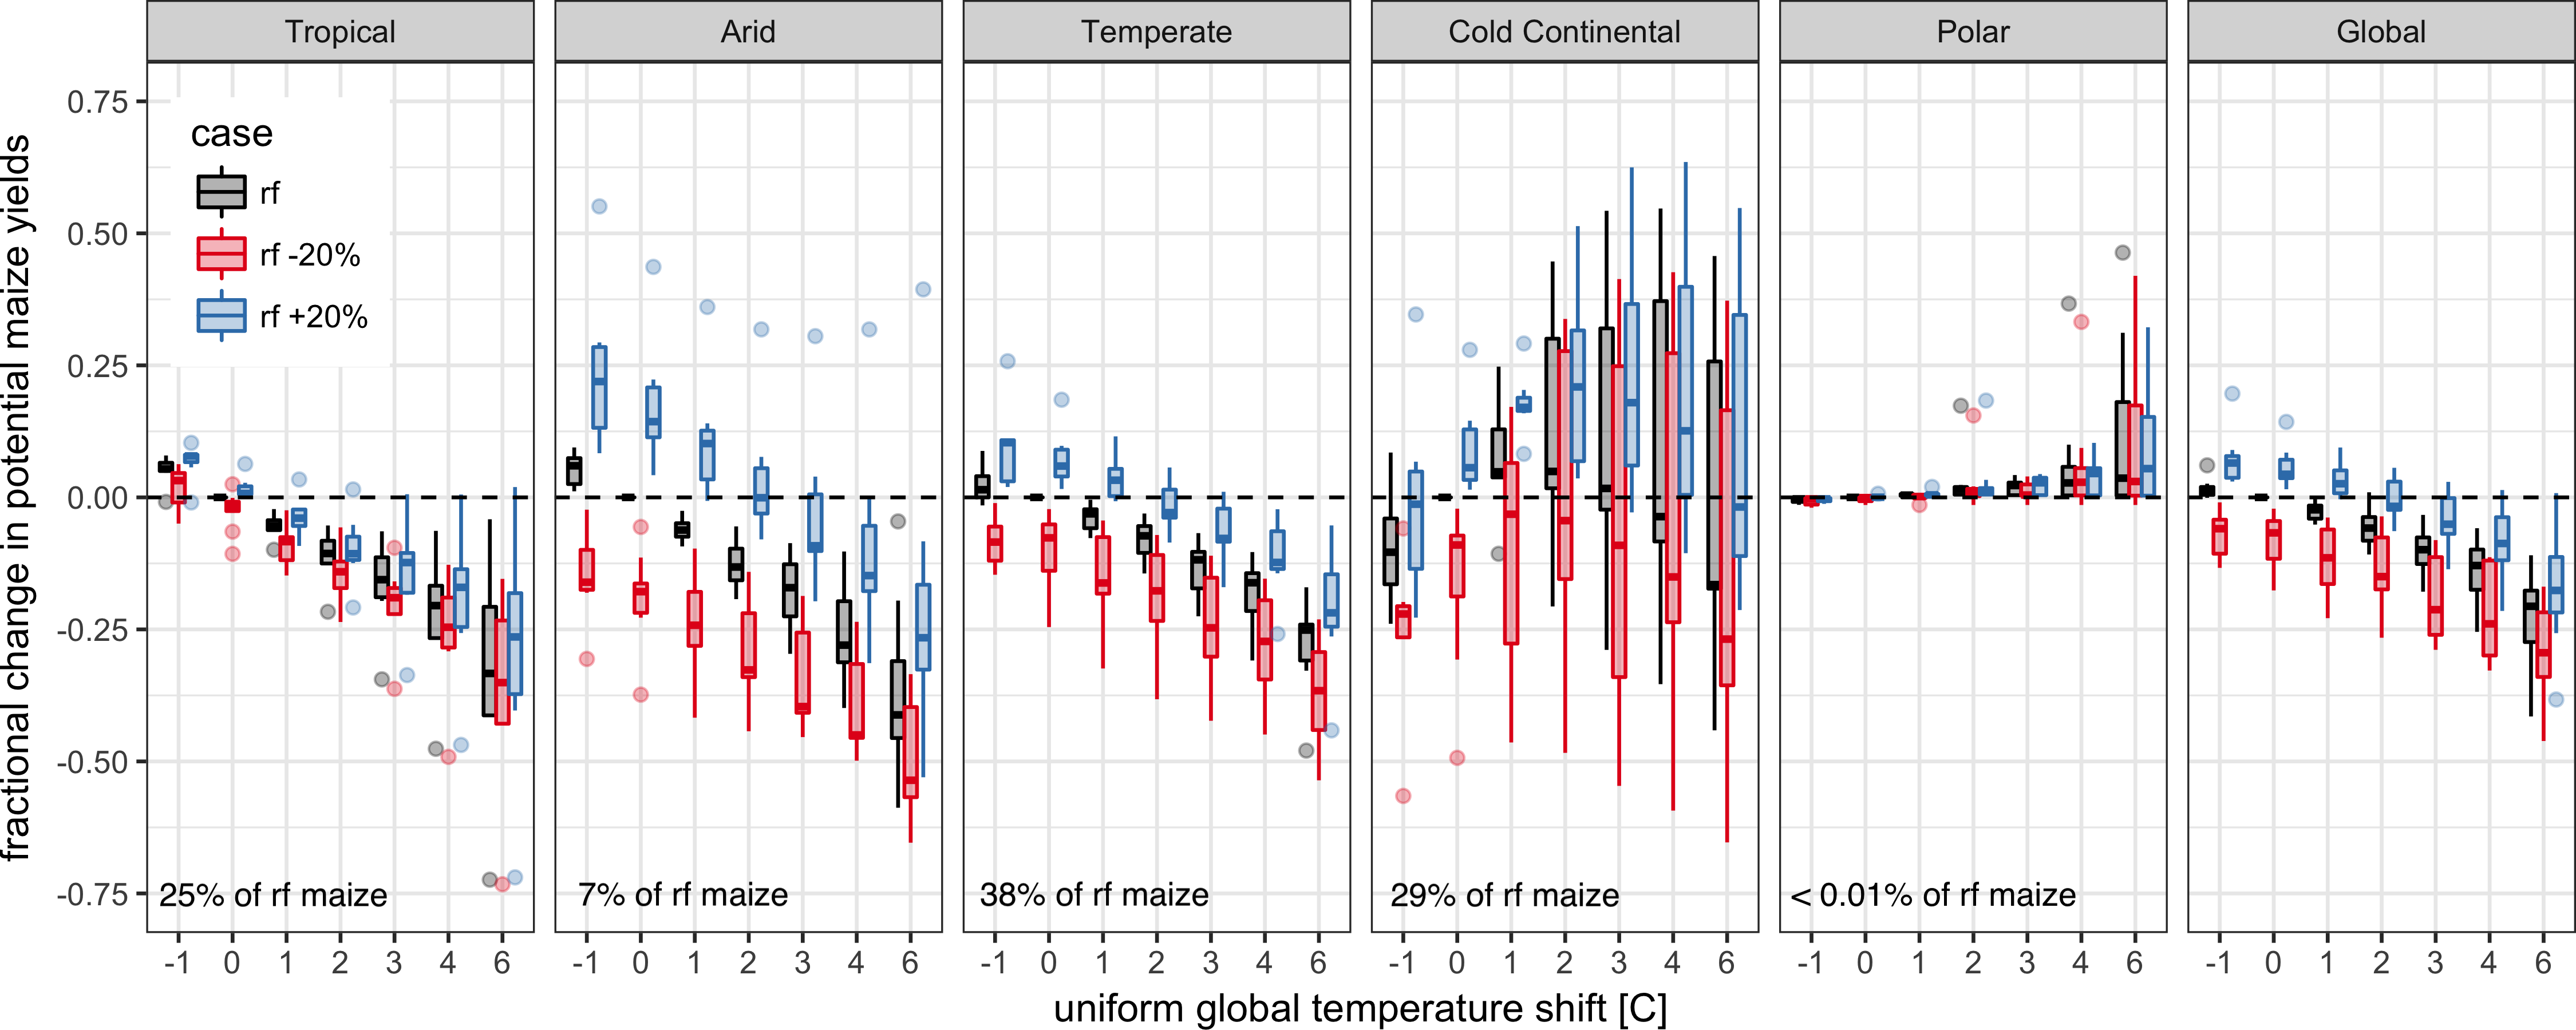
\includegraphics[width=0.99\linewidth]{figures/global_sim_CG.png}
   \caption{Illustration of the distribution of regional yield changes across the multi-model ensemble, split by K\"{o}ppen-Geiger climate regions (\cite{rubel2010}). We show responses of a single crop (rain-fed maize) to applied uniform temperature perturbations, for three discrete precipitation perturbation levels (rain-fed (rf) -20\%, rain-fed (0), and rain-fed +20\%), with CO$_2$ and nitrogen held constant at baseline values (360 pmm and 200 kg ha$^{-1}$ yr$^{-1}$). Y-axis is fractional change in the regional average climatological potential yield relative to the baseline. The figure shows all modeled land area; see Figure \ref{fig:KGirr_currentcult} in the supplemental material for only currently-cultivated land. Panel text gives the percentage of rain-fed maize presently cultivated in each climate zone \citep[data from][]{Portmann2010}. Box-and-whiskers plots show distribution across models, with median marked. Box edges are first and third quartiles, i.e.\ box height is the interquartile range (IQR). Whiskers extend to maximum and minimum of simulations but are limited at 1.5$\cdot$IQR; otherwise the outlier is shown. Models generally agree in most climate regions (other than cold continental), with projected changes larger than inter-model variance. Outliers in the tropics (strong negative impact of temperature increases) are the pDSSAT model; outliers in the high-rainfall case (strong positive impact of precipitation increases) are the JULES model. Inter-model variance increases in the case where precipitation is reduced, suggesting uncertainty in model response to water limitation. The right panel with global changes shows yield responses to an globally uniform temperature shift; note that these results are not directly comparable to simulations of more realistic climate scenarios with the same global mean change.}
   \label{fig:globesim}
\end{figure*}

The participating modeling groups provide simulations at any of four initially specified levels of participation, so the number of simulations varies by model, with some sampling only a part of the experiment variable space. Most modeling groups simulate all five crops in the protocol, but some omitted one or more. Table \ref{table:models} provides details of coverage for each model. Note that the three models that provide less than 50 simulations are excluded from the emulator analysis. 

Each model is run at 0.5 degree spatial resolution and covers all currently cultivated areas and much of the uncultivated land area. (See Figure \ref{fig:crop_area} for the present-day cultivated area of rain-fed crops, and Figure \ref{fig:irrarea} in the Supplemental Material for irrigated crops.)  Coverage extends considerably outside currently cultivated areas because cultivation will likely shift under climate change.  However, areas are not simulated if they are assumed to remain non-arable even under an extreme climate change; these regions include Greenland, far-northern Canada, Siberia, Antarctica, the Gobi and Sahara Deserts, and central Australia.  

All models produce as output crop yields (tons ha$^{-1}$ year$^{-1}$) for each 0.5 degree grid cell. Because both yields and yield changes vary substantially across models and across grid cells, we primarily analyze relative change from a baseline. We take as the baseline the scenario with historical climatology (i.e.\ T and P changes of 0), C of 360 ppm, and applied N at 200 kg ha$^-1$.  We show absolute yields in some cases to illustrate geographic differences in yields for a single model. 

\section{Simulation -- Results}
\label{S:3}

\begin{figure*}[!ht]
\centering
   \includegraphics[width=0.95\linewidth]{figures/baselinecomp_yield_3.png} 
   \caption{Illustration of the spatial pattern of potential yields and potential yield changes in the GGCMI Phase II ensemble, for three major crops. Left column (a) shows multi-model mean climatological yields for the baseline scenario for (top--bottom) rain-fed maize, soy, and rice. (For wheat see Figure \ref{fig:wheatbaseline} in the supplemental material.) White stippling indicates areas where these crops are not currently cultivated. Absence of cultivation aligns well with the lowest yield contour (0-2 ton ha$^{-1}$). Right column (b) shows the multi-model mean fractional yield change in the extreme T + 4 $^{\circ}$C scenario (with other inputs at baseline values). Areas without hatching or stippling are those where confidence in projections is high: the multi-model mean fractional change exceeds two standard deviations of the ensemble. ($\Delta > 2\sigma$). Hatching indicates areas of low confidence ($\Delta < 1 \sigma$), and stippling areas of medium confidence ($1 \sigma < \Delta < 2 \sigma$). Crop model results in cold areas, where yield impacts are on average positive, also have the highest uncertainty.}
   \label{fig:maizesoybaseline}
\end{figure*}

Crop models in the GGCMI Phase II ensemble show broadly consistent responses to climate and management perturbations in most regions, with a strong negative impact of increased temperature in all but the coldest regions. We illustrate this result for rain-fed maize in Figure \ref{fig:globesim}, which shows yields for the primary K\"{o}ppen-Geiger climate regions \citep{rubel2010}. In warming scenarios, models show decreases in maize yield in the warm temperate, equatorial, and arid regions that account for nearly three-quarters of global maize production. These impacts are robust for even moderate climate perturbations. In the warm temperate zone, even a 1 degree temperature rise with other variables held fixed leads to a median yield reduction that outweighs the variance across models. A 6 degree temperature rise results in median loss of $\sim$25\% of yields with a signal to noise ratio of nearly three to one. A notable exception is the snow region, where models disagree strongly, extending even to the sign of impacts. Other crops show similar responses to warming, with robust yield losses in warmer locations and high inter-model variance in the cold continental regions (Figure \ref{fig:KGcrops_all}).

The effects of rainfall changes on maize yields shown in  Figure \ref{fig:globesim} are also as expected and are consistent across models. Increased rainfall mitigates the negative effect of higher temperatures by counteracting the increased evapo-transpiration to some degree, most strongly in arid regions. Decreased rainfall amplifies yield losses and also increases inter-model variance more strongly, suggesting that models have difficulty representing crop response to water stress or increased evapo-transpiration due to warmer temperatures.  We show only rain-fed maize here; see Figure \ref{fig:KGirr_all} for the irrigated case. As expected, irrigated crops are more resilient to temperature increases in all regions, especially so where water is limiting.  

Mapping the distribution of baseline yields and yield changes shows the geographic dependencies that underlie these results. Figure \ref{fig:maizesoybaseline} shows baseline and changes in the T+4 scenario for rain-fed maize, soy, and rice in the multi-model ensemble mean, with locations of model agreement marked. Absolute yield potentials show strong spatial variation, with much of the Earth's surface area unsuitable for any given crop. In general, models agree most on yield response in regions where yield potentials are currently high and therefore where crops are currently grown. Models show robust decreases in yields at low latitudes, and highly uncertain median increases at most high latitudes. For wheat crops see Figure \ref{fig:wheatbaseline}; wheat projections are more uncertain potentially due to lack of calibration \citep[especially important for wheat][]{Asseng2013} and the more complicated phenological development of winter wheat when compared to other crops. Simulation model validation can be found in Appendix \ref{S:7}.

\section{Emulation -- Methods}
\label{S:4}
As part of our demonstration of the properties of the GGCMI Phase II dataset, we construct an emulator of 30-year climatological mean yields. This approach is made possible by the structured set of simulations involving systematic perturbations. %; training sets consisting of realistic, non-stationary scenarios generaly necessitate emulation at the annual level. %Annual emulation is required when the input training set consists of non-stationary projections of evolving yields (such as an RCP climate model run). 
%To demonstrate the utility of a climatological emulation approach, we use the 
In the GGCMI Phase II dataset, the year-over-year responses are generally quantitatively distinct from (and larger than) climatological mean responses. In the example of Figure \ref{fig:yearvclim}, responses to year-over-year temperature variations are 100\% larger than those to long-term perturbations in the baseline case, and larger still under warmer conditions, rising to nearly 200\% more in the T+6 case. The stronger year-over-year response under warmer conditions also manifests as a wider distribution of yields (Figure \ref{fig:yearly}).
As discussed previously, year-over-year and climatological responses can differ for many reasons including %year-to-year 
memory in the crop model, lurking covariants, and differing associated distributions of daily growing-season daily weather %associated with interannual variability is be different from that associated with long-term CO2-driven changes 
\citep[e.g.][]{Ruane2016}.
% shows that the year-over-year yield response to individual factors in GGCMI Phase II do in fact often exceed the climatological-mean response . 
Note that the GGCMI Phase II datasets do not capture one climatological factor, potential future distributional shifts, because all simulations are run with fixed offsets from the historical climatology. Prior work has suggested that mean changes are the dominant drivers of climatological crop yield shifts in non-arid regions \citep[e.g.][]{Glotter14}. 

% XXX --- save this for the discussion ---- For methods to generate adjust historical climate data inclusive of distributional and temporal dependence changes, see \citet{Leeds2015, poppick2016, Won16} and \citet{Haugen2018}). Emulation approaches are an area of active ongoing study and one of the goals of the GGCMI Phase II dataset is to facilitate these research efforts. 
\begin{figure}[th!]
\centering
   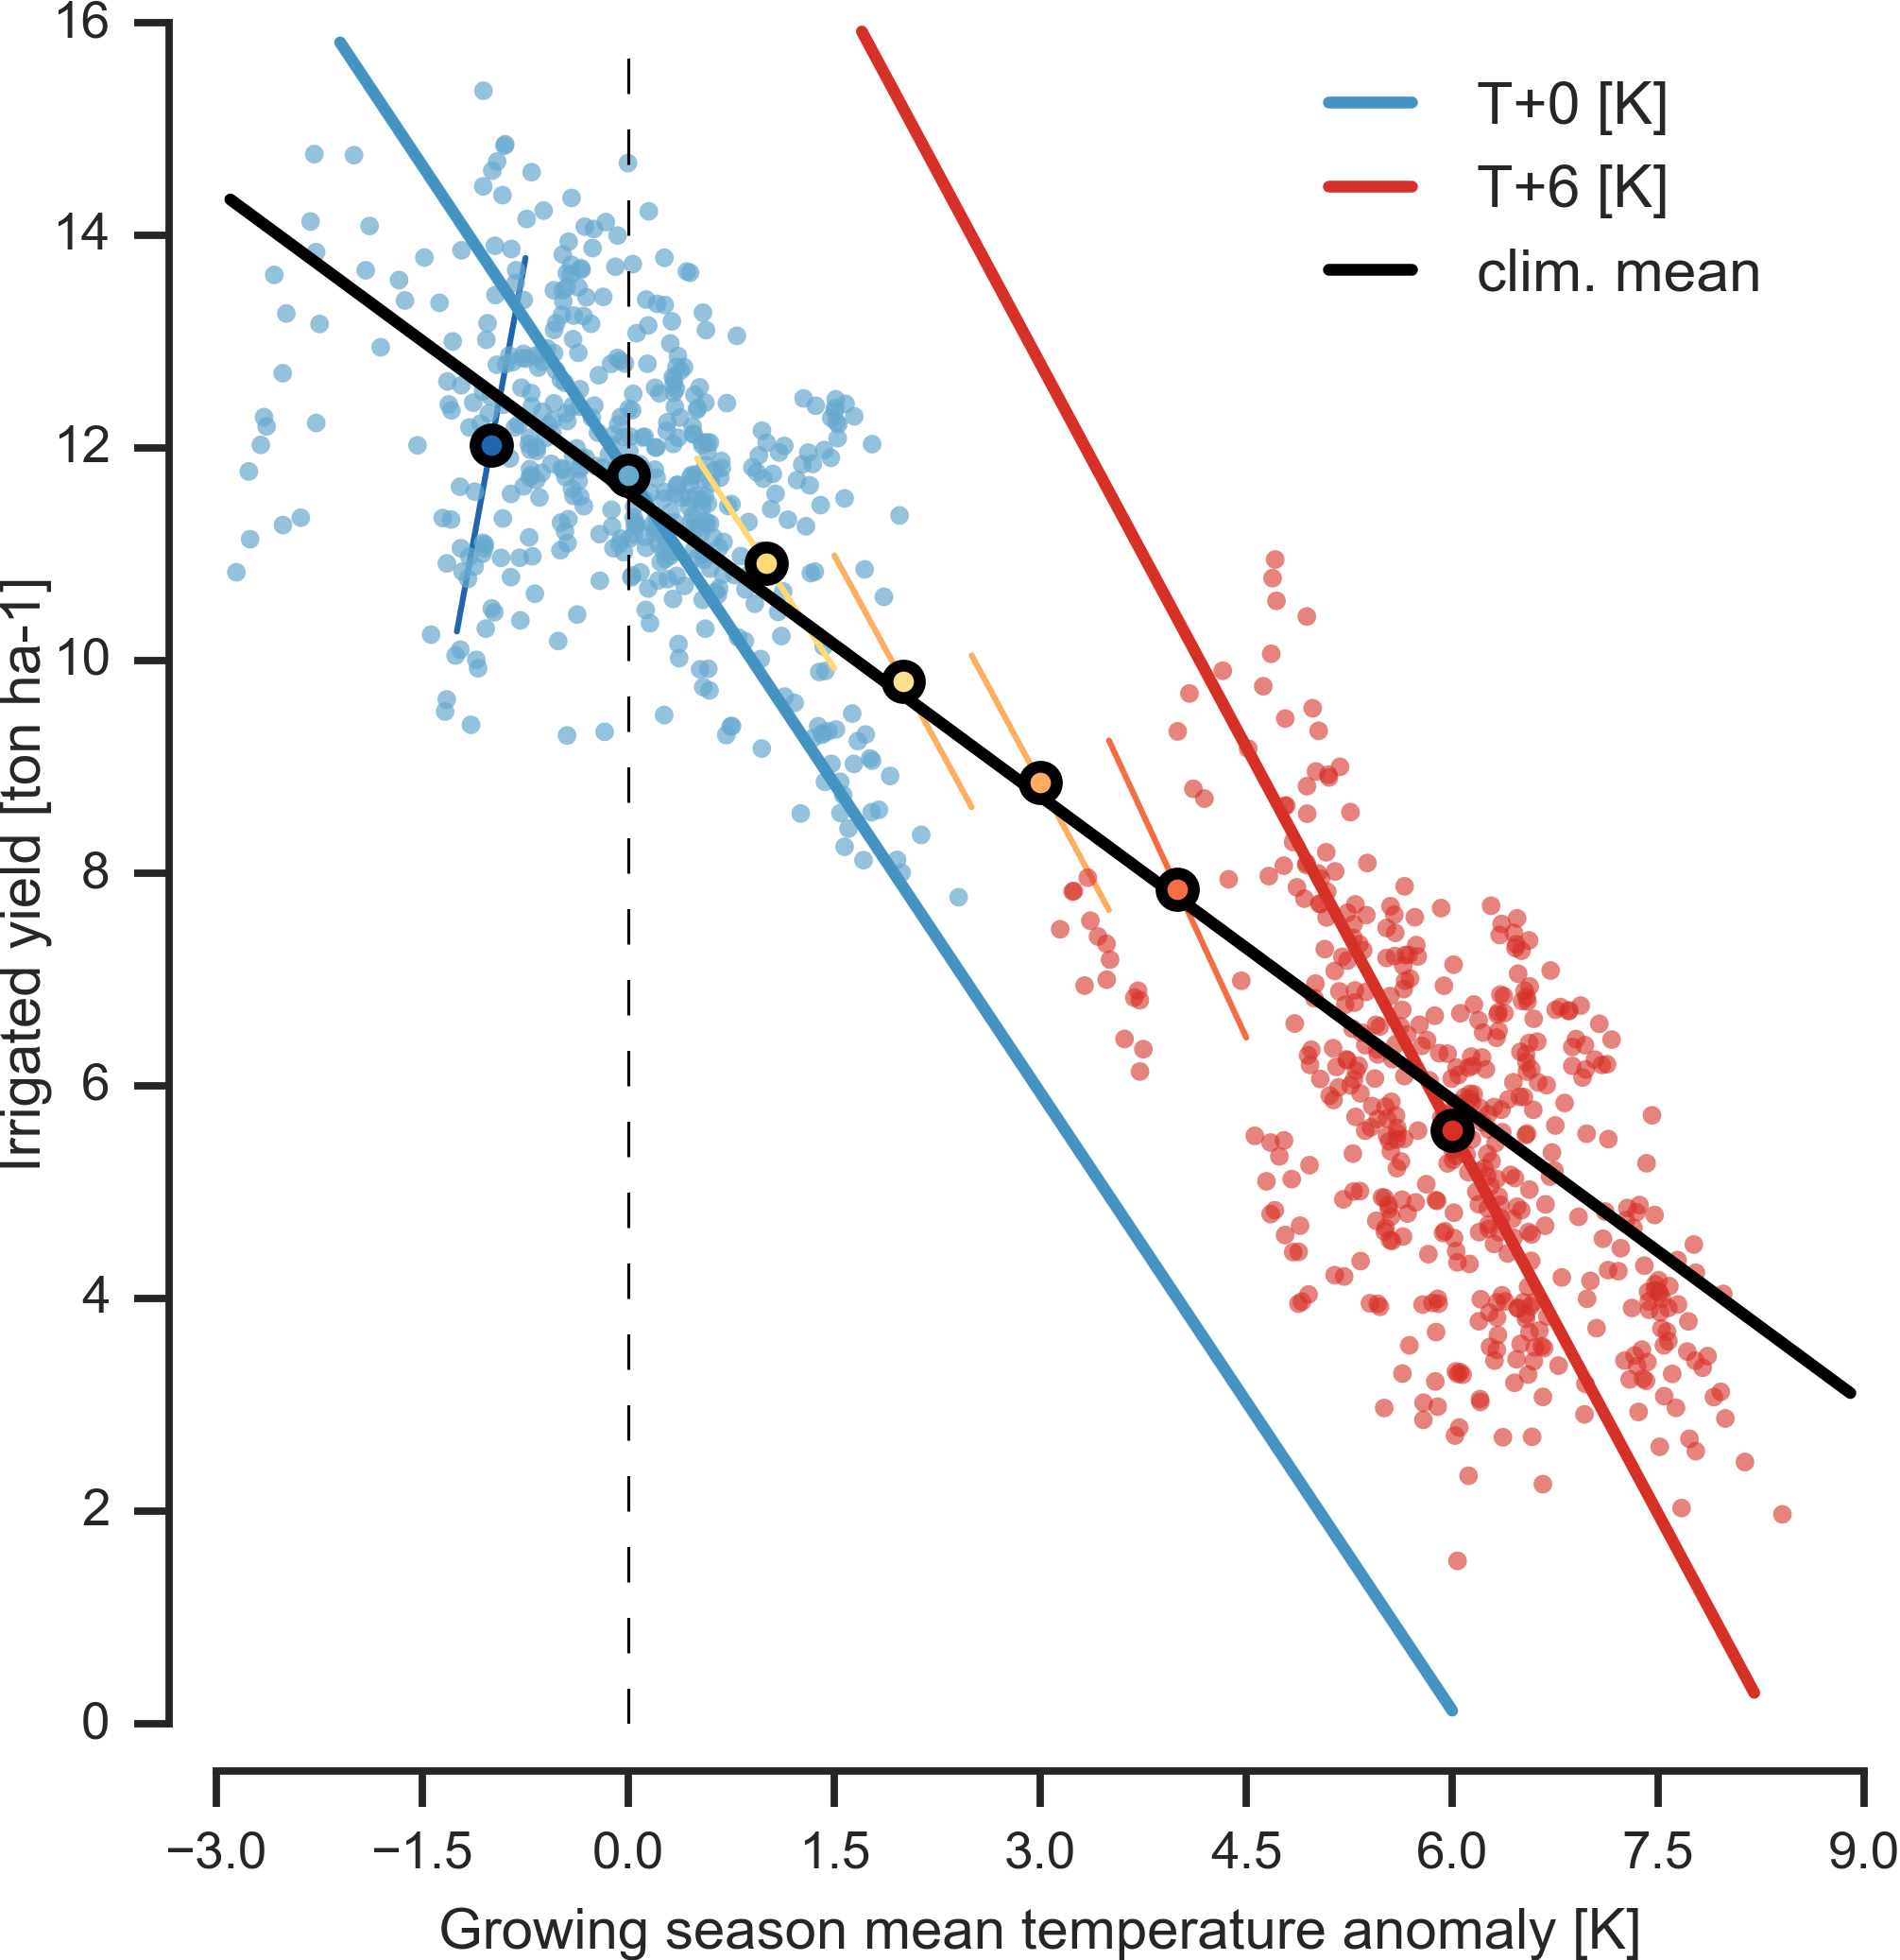
\includegraphics[width=0.95\linewidth]{figures/tempyearvclim.png}
   \caption{Example showing distinction between crop yield responses to year-to-year and climatological mean temperature shifts. Figure shows irrigated maize for a representative high-yield region (nine adjacent grid cells in northern Iowa) from the pDSSAT model, for the baseline 1981-2010 historical climate (blue) and for the scenario of maximum temperature change (+6 K, red). Other variables are held at baseline values, and the choice of irrigated yields means that precipitation is not a factor.   Open black circles mark climatological mean yield values for all six temperature scenarios (T-1, +0, +1, +2, +3, +4, +6). Colored lines show total least squares linear regressions of year-over-year variations in each scenario. Black line shows the fit through the climatological mean values.  Responses to year-over-year temperature variations (colored lines) are 100--200\% larger than those to long-term climate perturbations, rising under warmer conditions.}
   \label{fig:yearvclim}
\end{figure}

\begin{figure}[th!]
\centering
   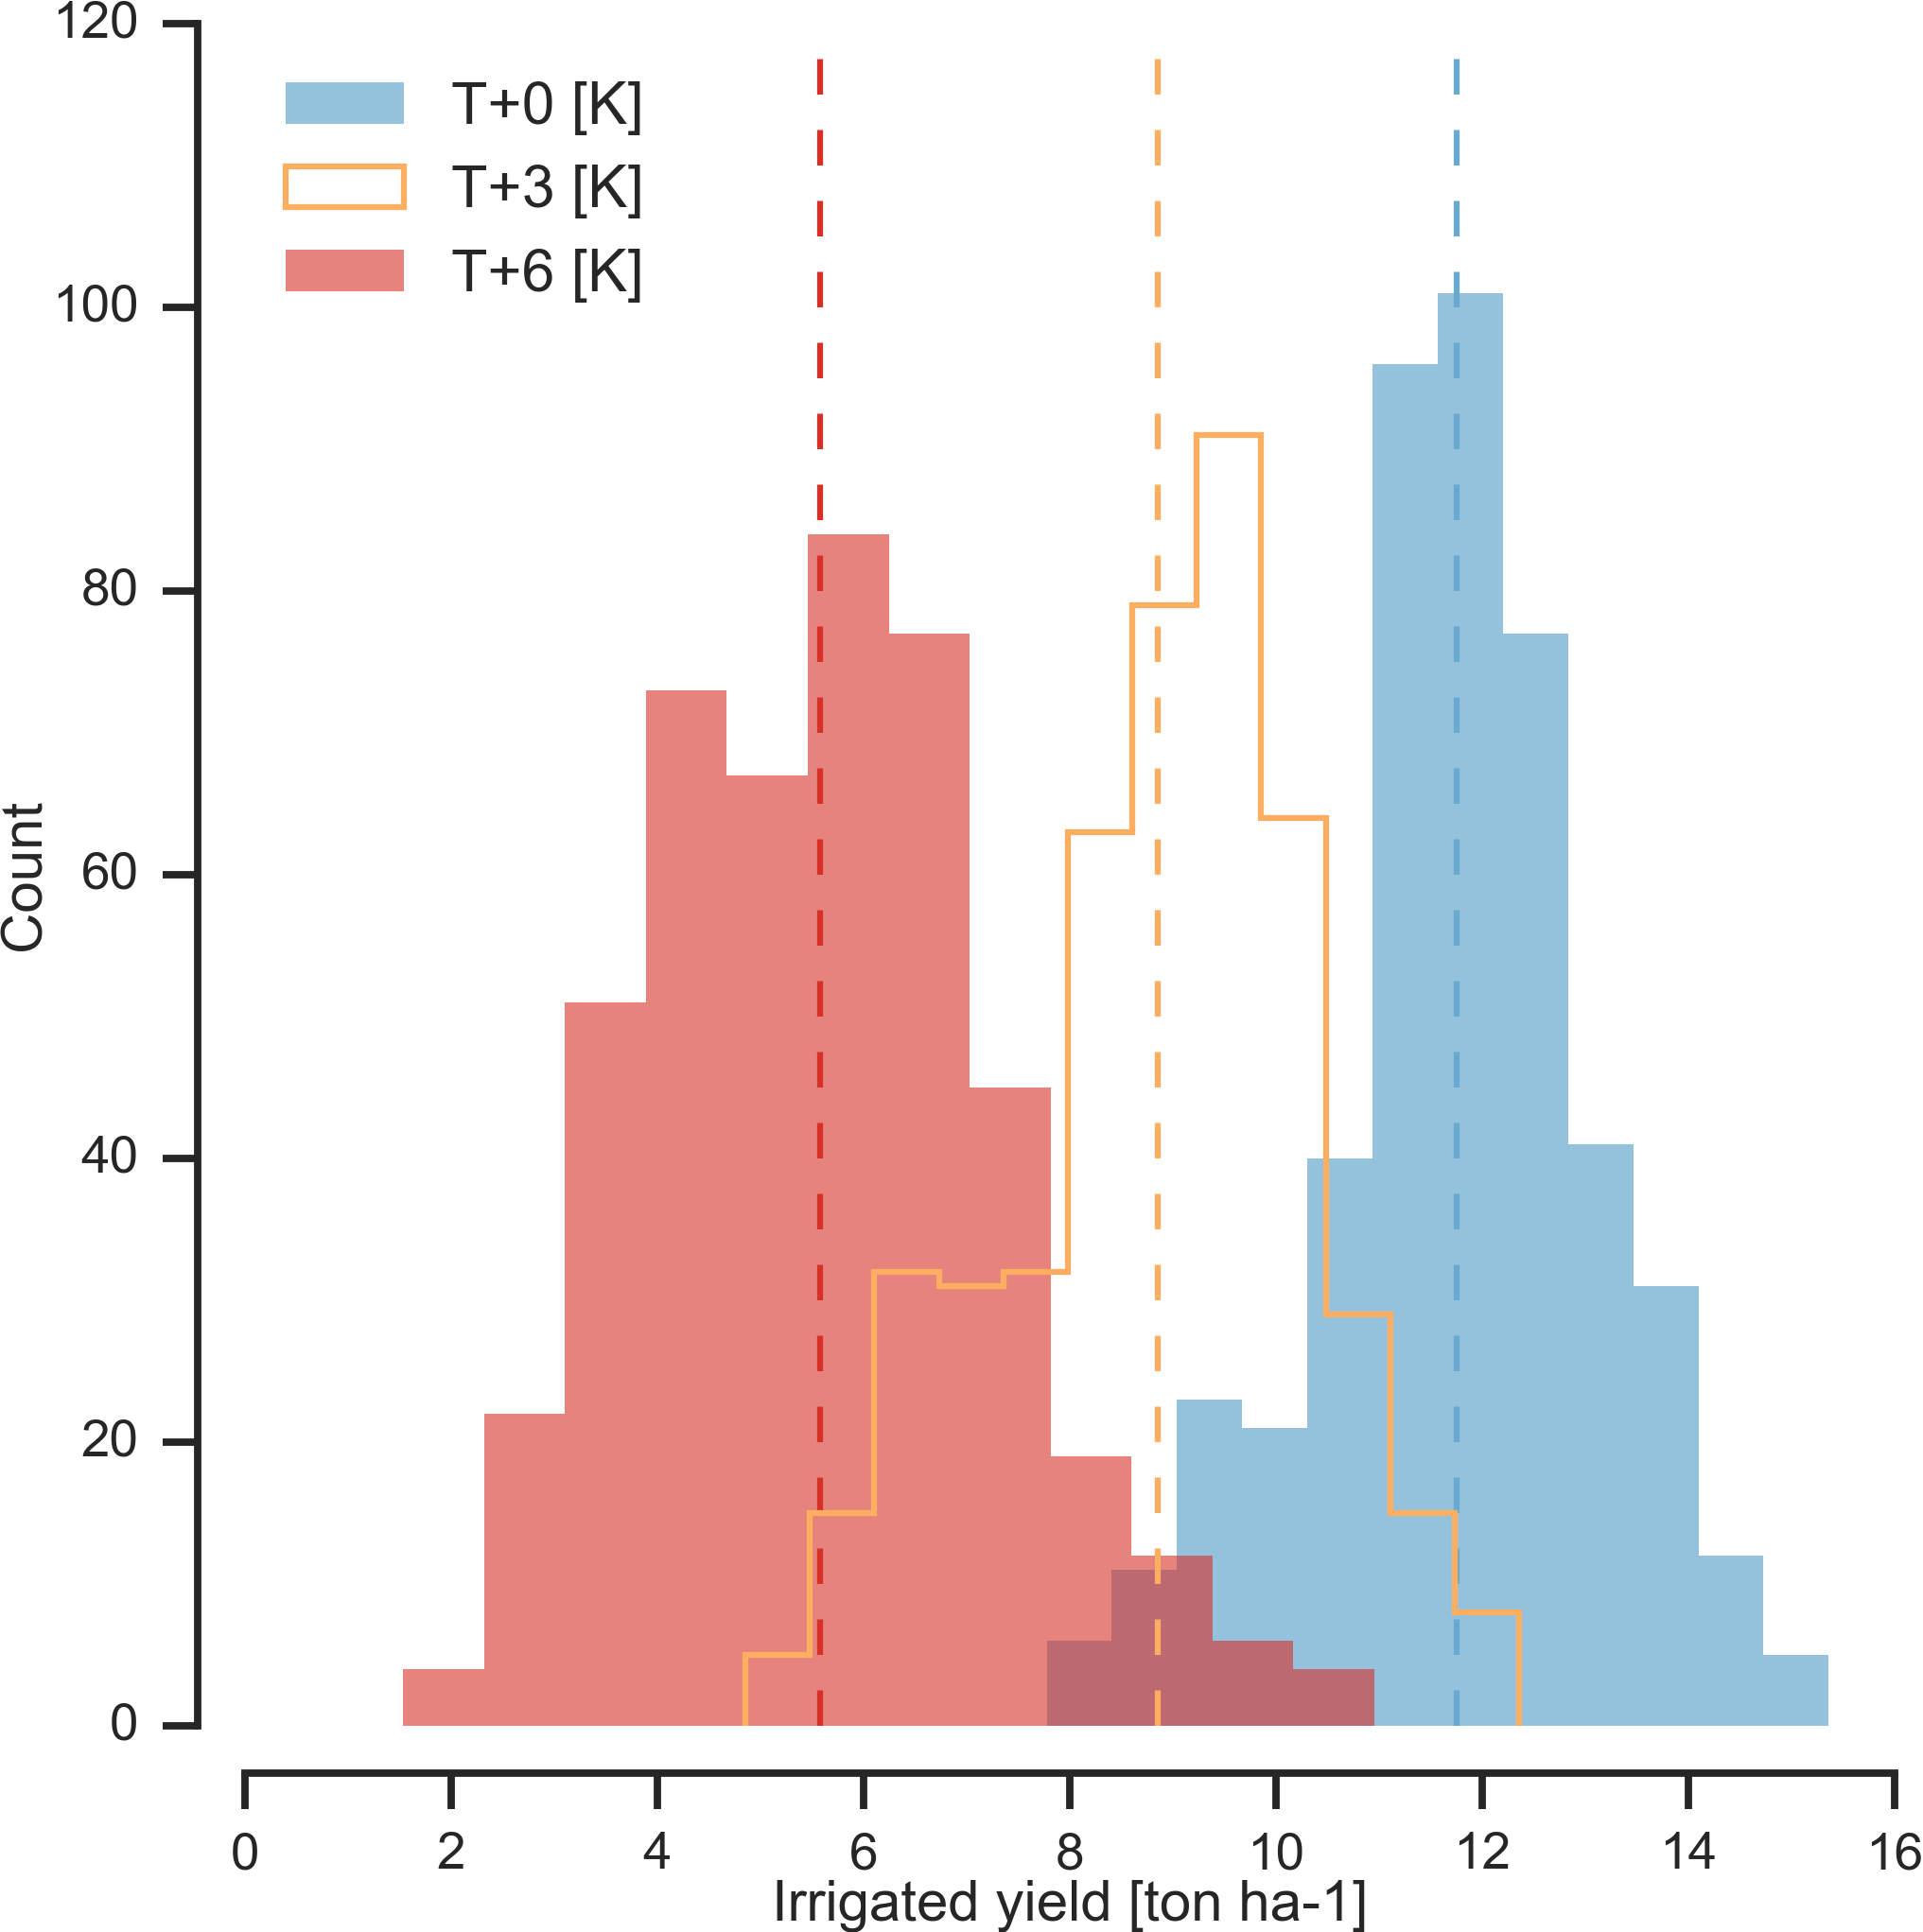
\includegraphics[width=0.95\linewidth]{figures/hist_year.png}
   \caption{Example showing climatological mean yields and distribution of yearly yields for three 30-year scenarios. Figure shows irragated maize for nine adjacent high-yield grid cells of Figure \ref{fig:yearvclim} (in northern Iowa, same as Figure \ref{fig:yearvclim}) from the pDSSAT model, for the baseline 1981-2010 historical climate (blue) and for scenarios with temperature shifted by T+3 (orange) and T+6 K (red), with other variables held at baseline values. The stronger year-over-year temperature response with higher temperatures seen in Figure \ref{fig:yearvclim} is manifested here as larger variance in annual yields. In this work we emulate not the year-over-year distributions but the climatological mean response (dashed vertical lines).}
   \label{fig:yearly}
\end{figure}

Emulation involves fitting individual regression models for each crop, simulation model, and 0.5 degree geographic pixel from the GGCMI Phase II dataset; the regressors are the applied constant perturbations in CO$_2$, temperature, water, and nitrogen (C,T, W, N).  We regress 30-year climatological mean yields against a third-order polynomial in C, T, W, and N with interaction terms. (We aggregate the entire 30-year run in each case to improve signal to noise ration in our model.) The higher-order terms are necessary to capture any nonlinear responses, which are well-documented in observations for temperature and water perturbations (e.g.\ \citet{Schlenker2009} for T and \citet{He2016} for W). We include interaction terms (both linear and higher-order) because past studies have shown them to be significant effects. For example, \citet{Lobell2007} and \citet{Tebaldi2008} showed that in real-world yields, the joint distribution in T and W is needed to explain observed yield variance. (C and N are fixed in these data.) Other observation-based studies have shown the importance of the interaction between water and nitrogen \citep[e.g.][]{AULAKH2005}, and between nitrogen and carbon dioxide \citep{Mitsuru92, Nakamura97}. To avoid overfitting or unstable parameter estimation, we apply a feature selection procedure (described below) that reduces the potential 34-term polynomial (for the rain-fed case) to 23 terms.

We do not focus on comparing different functional forms in this study, and instead choose a relatively simple parametrization that allows for some interpretation of coefficients. Some prior studies have used more complex functional forms and larger numbers of parameters, e.g.\ 39 in \citet{BLANC2015} and \citet{BLANC2017}, who borrow information across space by fitting grid points simultaneously across a large region in a panel regression.
We do not aggregate in space since the emulation is not computationally demanding even at the half-degree grid cell resolution globally. 
The emulation therefore indirectly includes any yield response to geographically distributed factors such as soil type, insolation, and the baseline climate itself. We explicitly hold the statistical specification constant across all crops and models to facilitate model comparison by looking at parameters directly in lieu of the much larger yield output space.

{\color{red} The relatively simple functional form used here allows emulation at grid-cell level with low noise? how do you quantify this?

maybe add table of parameters like stefan said?}


We do not focus on comparing different functional forms in this study, and instead choose a relatively simple parametrization that allows for some interpretation of coefficients. Some prior studies have used more complex functional forms and larger numbers of parameters, e.g.\ 39 in \citet{BLANC2015} and \citet{BLANC2017}, who borrow information across space by fitting grid points simultaneously across a large region in a panel regression.
%We do not aggregate in space since the emulation is not computationally demanding  even at the half-degree grid cell resolution 
 The simpler functional form used here allows emulation at grid-cell level {\color{red} with low noise? how do you quantify this?}. 
The emulation therefore indirectly includes any yield response to geographically distributed factors such as soil type, insolation, and the baseline climate itself. 

%The regression therefore omits information about yield responses to year-to-year climate perturbations, which are more complex. Emulating inter-annual yield variations would likely require considering statistical details of the historical climate time series, including changes in marginal distribution and temporal dependencies. (Future work should explore this). 

%Crop yields in process based models do not respond to the mean growing season temperature, they respond the the full distribution in temperature over the growing season (or, specifically the exact temperature time series). Much of the variance is left unexplained if one tries to fit a statistical model between yields and some aggregate temperature variable (mean growing season temperature, monthly temperature etc.).

\subsection{Feature selection procedure}
Although the GGCMI Phase II sampled variable space is large, it is still sufficiently limited that use of the full polynomial expression described above can be problematic. %, and can lead to over-fitting and unstable parameter estimations. 
We therefore reduce the number of terms through a feature selection cross-validation process in which terms in the polynomial are tested for importance. In this procedure higher-order and interaction terms are added successively to the model; we then follow the reduction of the the aggregate mean squared error with increasing terms and eliminate those terms that do not contribute significant reductions. See supplemental documents for more details. We select terms by applying the feature selection process to the three models that provided the complete set of 672 rain-fed simulations (pDSSAT, EPIC-TAMU, and LPJmL); the resulting choice of terms is then applied for all emulators. 

\begin{figure*}[!hb]
\centering
    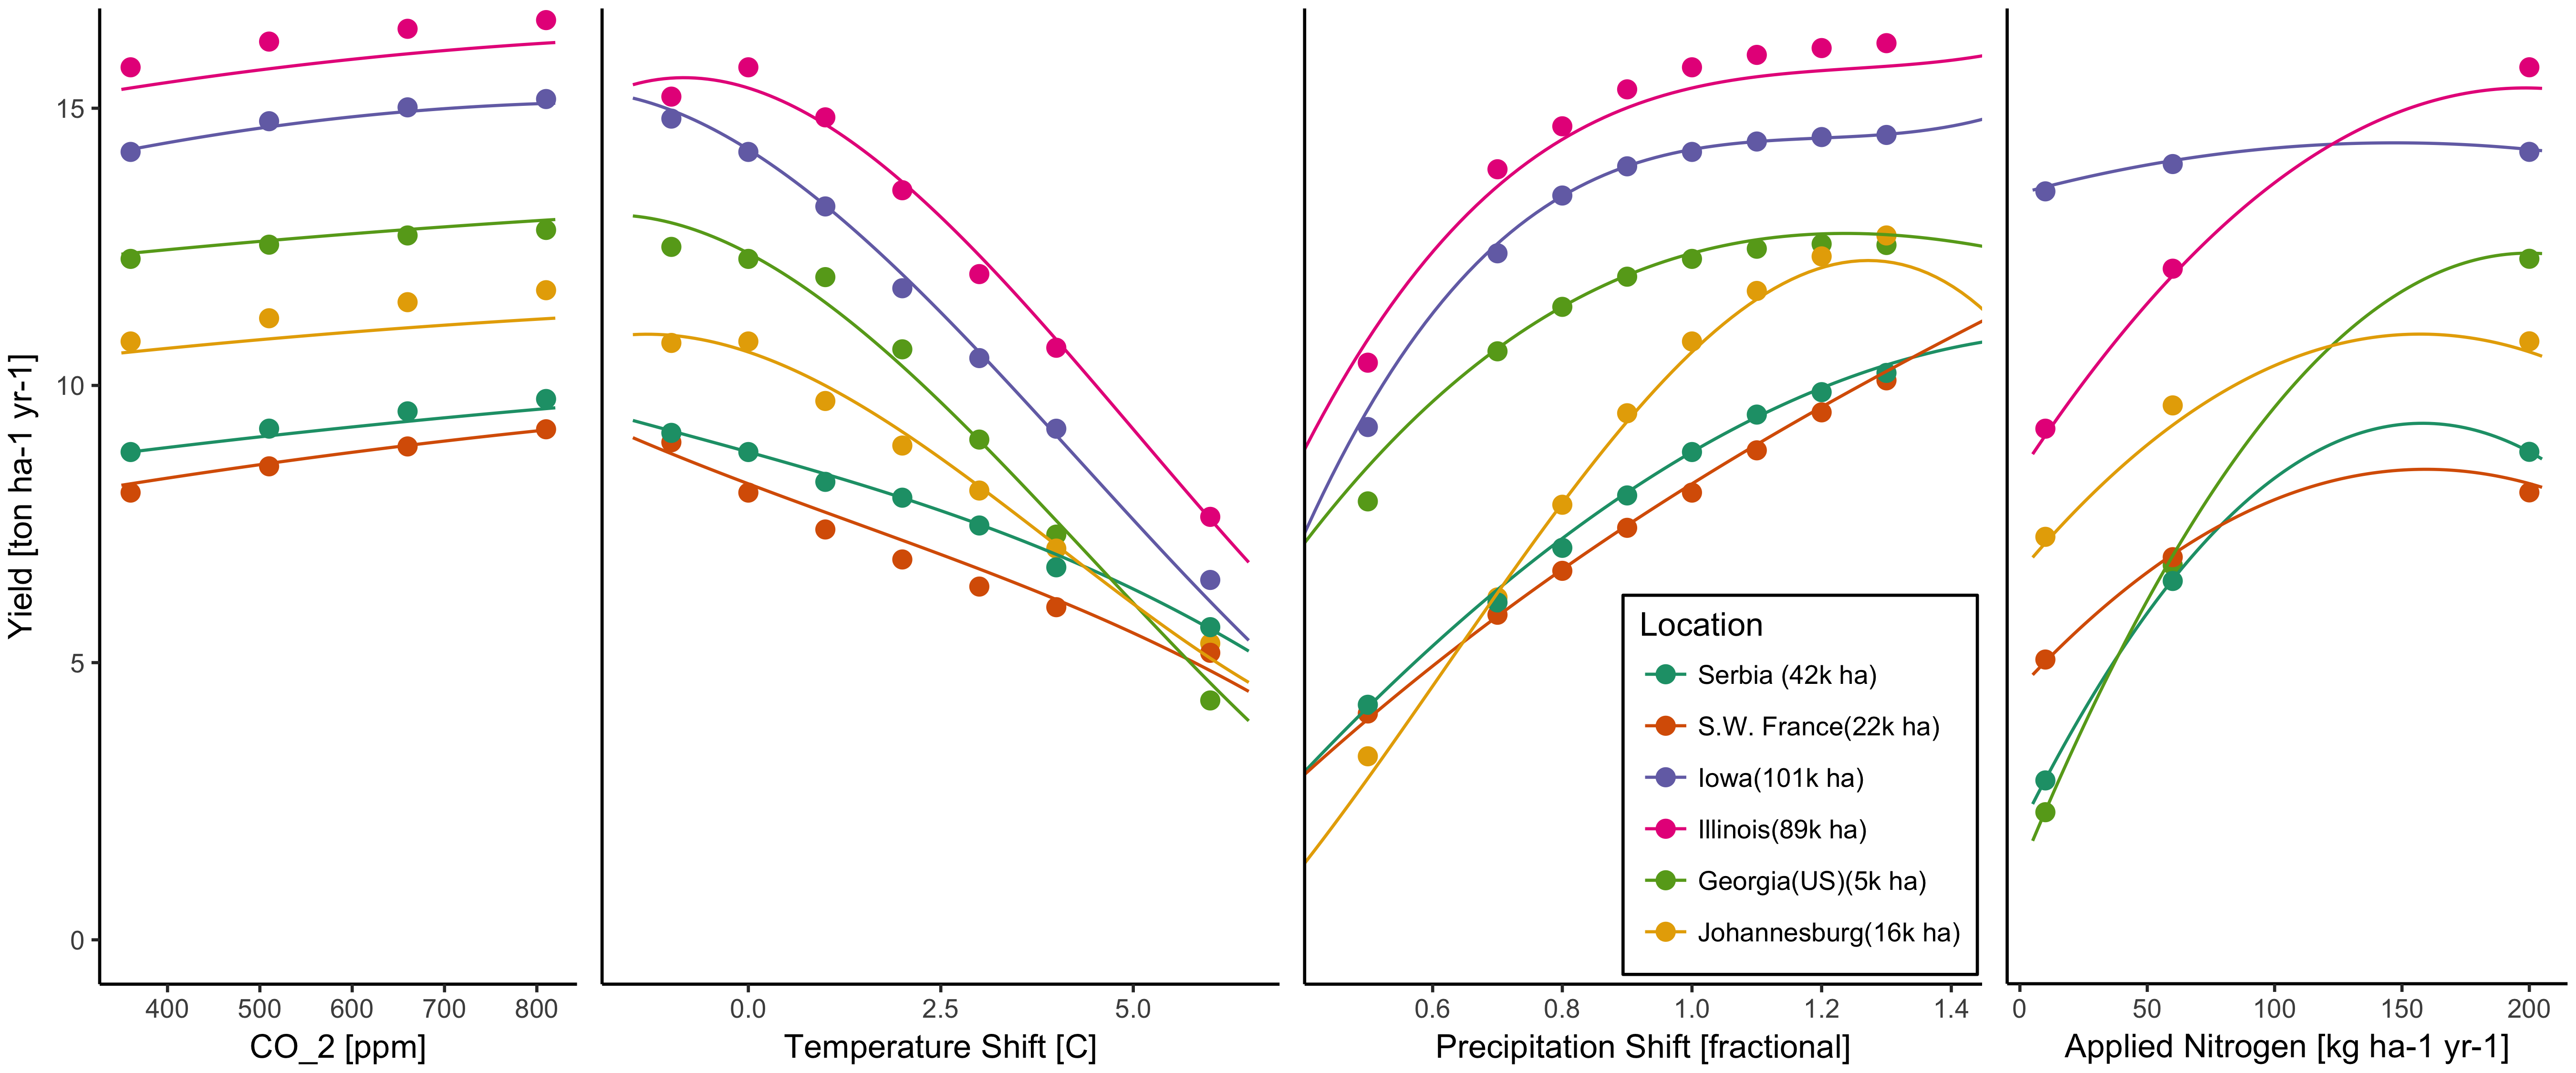
\includegraphics[width=0.95\linewidth]{figures/regression_areas.png}
    \caption{Illustration of spatial variations in yield response and emulation ability. We show rain-fed maize in the pDSSAT model in six example locations selected to represent high-cultivation areas around the globe. Legend includes hectares cultivated in each selected grid cell. Each panel shows variation along a single variable, with others held at baseline values. Dots show climatological mean yields  
%solid lines a simple polynomial fit across this 1D variation, 
and lines the results of the full 4D emulator of Equation \ref{eqn:features_final}. In general the climatological response surface is sufficiently smooth that it can be represented with the sampled variable space by the simple polynomial used in this work. Extrapolation can however produce misleading results. Nitrogen fits may not be realistic at intermediate values given limited sampling. For more detailed emulator assessment, see Appendix \ref{S:8}. %Note that because precipitation changes are imposed as multiplicative factors rather than additive offsets, locations with higher baseline precipitation have a larger absolute spread in inputs sampled than do drier locations (not visible here).
}
   \label{fig:regression}
\end{figure*}

Feature importance is remarkably consistent across all three models and across all crops (see Figure \ref{fig:featureselection} in the supplemental material). The feature selection process results in a final polynomial in 23 terms, with 11 terms eliminated. We omit the N$^3$ term, which cannot be fitted because we sample only three nitrogen levels. We eliminate many of the C terms: the cubic, the CT, CTN, and CWN interaction terms, and all higher order interaction terms in C. Finally, we eliminate two 2nd-order interaction terms in T and one in W. Implication of this choice include that nitrogen interactions are complex and important, and that water interaction effects are more nonlinear than those in temperature. The resulting statistical model (Equation \ref{eqn:features_final}) is used for all grid cells, models, and rain-fed crops. The regression for irrigated crops does not contain the W terms and models that did not sample the nitrogen levels (see \ref{table:models} do not contain any of the N terms.
\begin{align}
    \label{eqn:features_final}
    Y\ = \ & K_{1}  \\
       + \ & K_{2}  C     + K_{3}  T     + K_{4}  W     + K_{5}  N   \nonumber \\
       + \ & K_{6}  C^2   + K_{7}  T^2   + K_{8}  W^2   + K_{9}  N^2 \nonumber \\
       + \ & K_{10} C W   + K_{11} C N   + K_{12} T W   + K_{13} T N + K_{14} W N \nonumber \\ % lost 1 term, CT
       + \ & K_{15} T^3   + K_{16} W^3   + K_{17} T W N  \nonumber \\ % lost 2 terms, C^3 and N^3
       + \ & K_{18} T^2 W + K_{19} W^2 T + K_{20} W^2 N  \nonumber \\ % lost 2 terms, CWN and CTN
       + \ & K_{21} N^2 C + K_{22} N^2 T + K_{23} N^2 W  \nonumber    % lose 6 terms: T^2N and T^2C, W^2C, 3 C^2 terms
\end{align}

To fit the parameters $K$, we use a Bayesian Ridge probabilistic estimator \citep{MacKay91}, which reduces volatility in parameter estimates when the sampling is sparse, by weighting parameter estimates towards zero. The Bayesian Ridge method is necessary to maintain a consistent functional form across all models and locations. % as the linear least squares fails to provide a stable result in many cases.
 We use the implementation of the Bayesian Ridge estimator from the scikit-learn package in Python \citep{scikit-learn}. 
In the GGCMI Phase II experiment, the most problematic fits are those for models that provided a limited number of cases or for low-yield geographic regions where some modeling groups did not run all scenarios. We do not attempt to emulate models that provided less than 50 simulations. The lowest number of simulations emulated across the full parameter space is then 130 (for the PEPIC model). 
The resulting parameter matrices for all crop model emulators are available on request {\color{red} give location?}, as are the raw simulation data and a Python application to emulate yields. The yield output for a single GGCMI Phase II model that simulates all scenarios and all five crops is $\sim$12.5 GB; the emulator is $\sim$100 MB, a reduction by over two orders of magnitude. 


\begin{figure*}[!!h]
\centering
    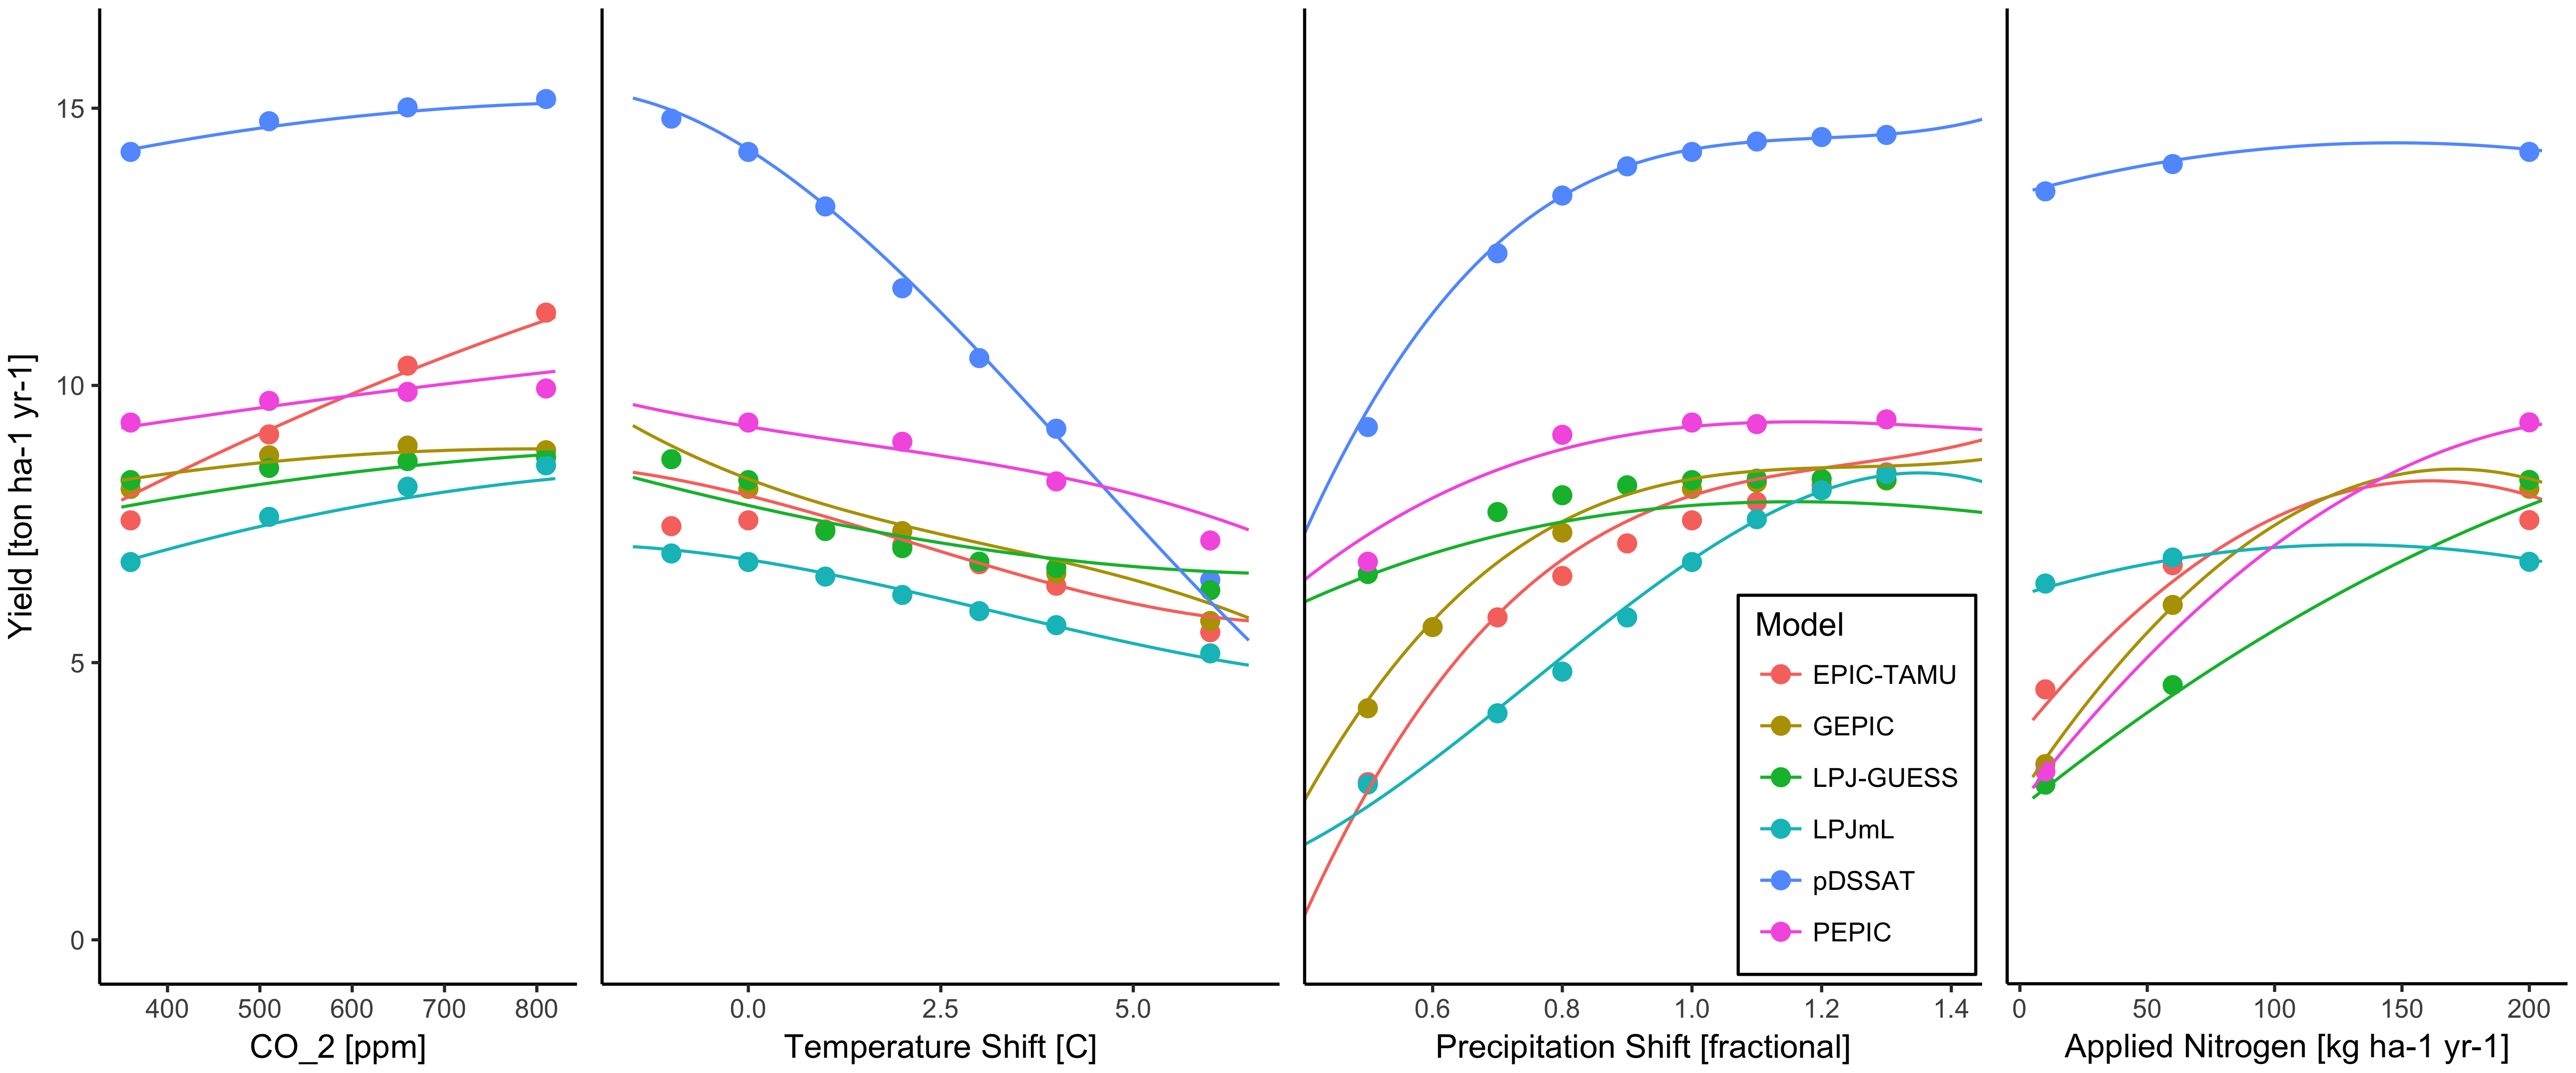
\includegraphics[width=0.95\linewidth]{figures/regression_model.png}
    \caption{Illustration of across-model variations in yield response. Figures shows simulations and emulations from six models for rain-fed maize in the same Iowa grid cell shown in Figure \ref{fig:regression}, with the same plot conventions. Models that do not simulate the nitrogen dimension are omitted for clarity. Note that models are uncalibrated, increasing spread in absolute yields.  %The inter-model standard deviation is larger for the perturbations in CO$_2$ and nitrogen than for those in temperature or precipitation illustrating that the sensitivity to weather is better constrained than to management at elevated CO$_2$. 
While most model responses can readily emulated with a simple polynomial, some response surfaces are more complicated (e.g.\  LPJ-GUESS here) and lead to emulation error, though error generally remains small relative to inter-model uncertainty. For more detailed emulator assessment, see Appendix \ref{S:8}. As in Figure \ref{fig:regression}, extrapolation out of the sample space is problematic. 
}
   \label{fig:regression_iowa}
\end{figure*}


\section{Emulation -- Results}
\label{S:5}
Emulation provides not only a computational tool but a means of understanding and interpreting crop yield response across the parameter space. Emulation is only possible  when crop yield responses are sufficiently smooth and continuous to allow fitting with a relatively simple functional form, but this condition largely holds in the GGCMI Phase II simulations. 
Responses are quite diverse across locations, crops, and models, but in most cases local responses are regular enough to permit emulation. We show illustrations of emulation fidelity in this section; for more detailed discussion see Appendix \ref{S:8}.

Crop yield responses are geographically diverse, even in high-yield and high-cultivation areas  
Figure \ref{fig:regression} illustrates geographic diversity for a single crop and model (rain-fed maize in pDSSAT); this heterogeneity supports the choice of emulating at the grid cell level. 
Each panel in Figure \ref{fig:regression} shows simulated yield output from scenarios varying only along a single dimension (CO$_2$, temperature, precipitation, or nitrogen addition), with other inputs held fixed at baseline levels, compared to the full 4D emulation across the parameter space. 
Yields evolve smoothly across the space sampled, and the polynomial fit captures the climatological response to perturbations.
Crop yield responses generally follow similar functional forms across models, though with a large spread in magnitude likely due to the lack of calibration. Figure \ref{fig:regression_iowa} illustrates inter-model diversity for a single crop and location (rain-fed maize in northern Iowa, also shown in Figure \ref{fig:regression}). %The differences make it important to construct emulators separately for each individual model, and 
Differences in response shape can lead to  differences in the fidelity of emulation, though comparison here is complicated by the different sampling regimes across models. Note that models are most similar in their responses to temperature perturbations. 
%This figure illustrates a common phenomenon, that models differ more in response to perturbations in CO$_2$ and nitrogen perturbations than to those in temperature or precipitation. (Compare also Figures \ref{fig:globesim} and \ref{fig:carbon}.) 
For this location and crop, {\color{red}CO$_2$ fertilization effects can range from $\sim$5--50\%}, and nitrogen responses from nearly flat to a 60\% drop in the lowest-application simulation. 

This is subject to large uncertainties, because not all relevant processes have been studied in sufficient detail or have not been implemented in models sufficiently \citep[e.g.][](e.g. Long et al. 2006, Boote et al. 2013) and a broader experimental basis for model parameterization is needed \citep{leaky09}. 

While the nitrogen dimension is important, it is also the most problematic to emulate in this work because of its limited sampling. The GGCMI Phase II protocol specified only three nitrogen levels (10, 60 and 200 kg~N y$^{-1}$ ha$^{-1}$), so a third-order fit would be over-determined but a second-order fit can result in potentially unphysical results. Steep and nonlinear declines in yield with lower nitrogen levels mean that some regressions imply a peak in yield between the 100 and 200 kg~N y$^{-1}$ ha$^{-1}$ levels. While it is possible that over-application of nitrogen at the wrong time in the growing season could lead to reduced yields, these features are potentially an artifact of undersampling. In addition, the polynomial fit cannot capture the well-documented saturation effect of nitrogen application \citep[e.g.][]{Torsten77} as accurately as would be possible with a non-parametric model. 

%\subsection{Emulator applications}
The emulation fidelity demonstrated here is sufficient to allow using emulated response surfaces to compare model responses and derive insight about impacts projections. 
Because the emulator or ``surrogate model'' transforms the discrete simulation sample space into a continuous response surface at any geographic scale, it can be used for a variety of applications, including construction of continuous damage functions. As an example, we show a damage function constructed from the 4D emulation, aggregated to global yield, with simulated values shown for comparison (Figure \ref{fig:globe_em}, which shows maize on currently cultivated land; see Figures \ref{fig:temperature}- \ref{fig:nitrogen} for other crops and dimensions). The emulated values closely match simulations even at this aggregation level. Note that these functions are presented only as examples and do not represent true global projections, because they are developed from simulation data with a uniform temperature shift while increases in global mean temperature should manifest non-uniformly. The global coverage of the GGCMI Phase II simulations allows impacts modelers to apply arbitrary geographically-varying climate projections, as well as arbitrary aggregation masks, to develop damage functions for any climate scenario and any geopolitical or geographic level.

\begin{figure}[!htb]
    \centering
    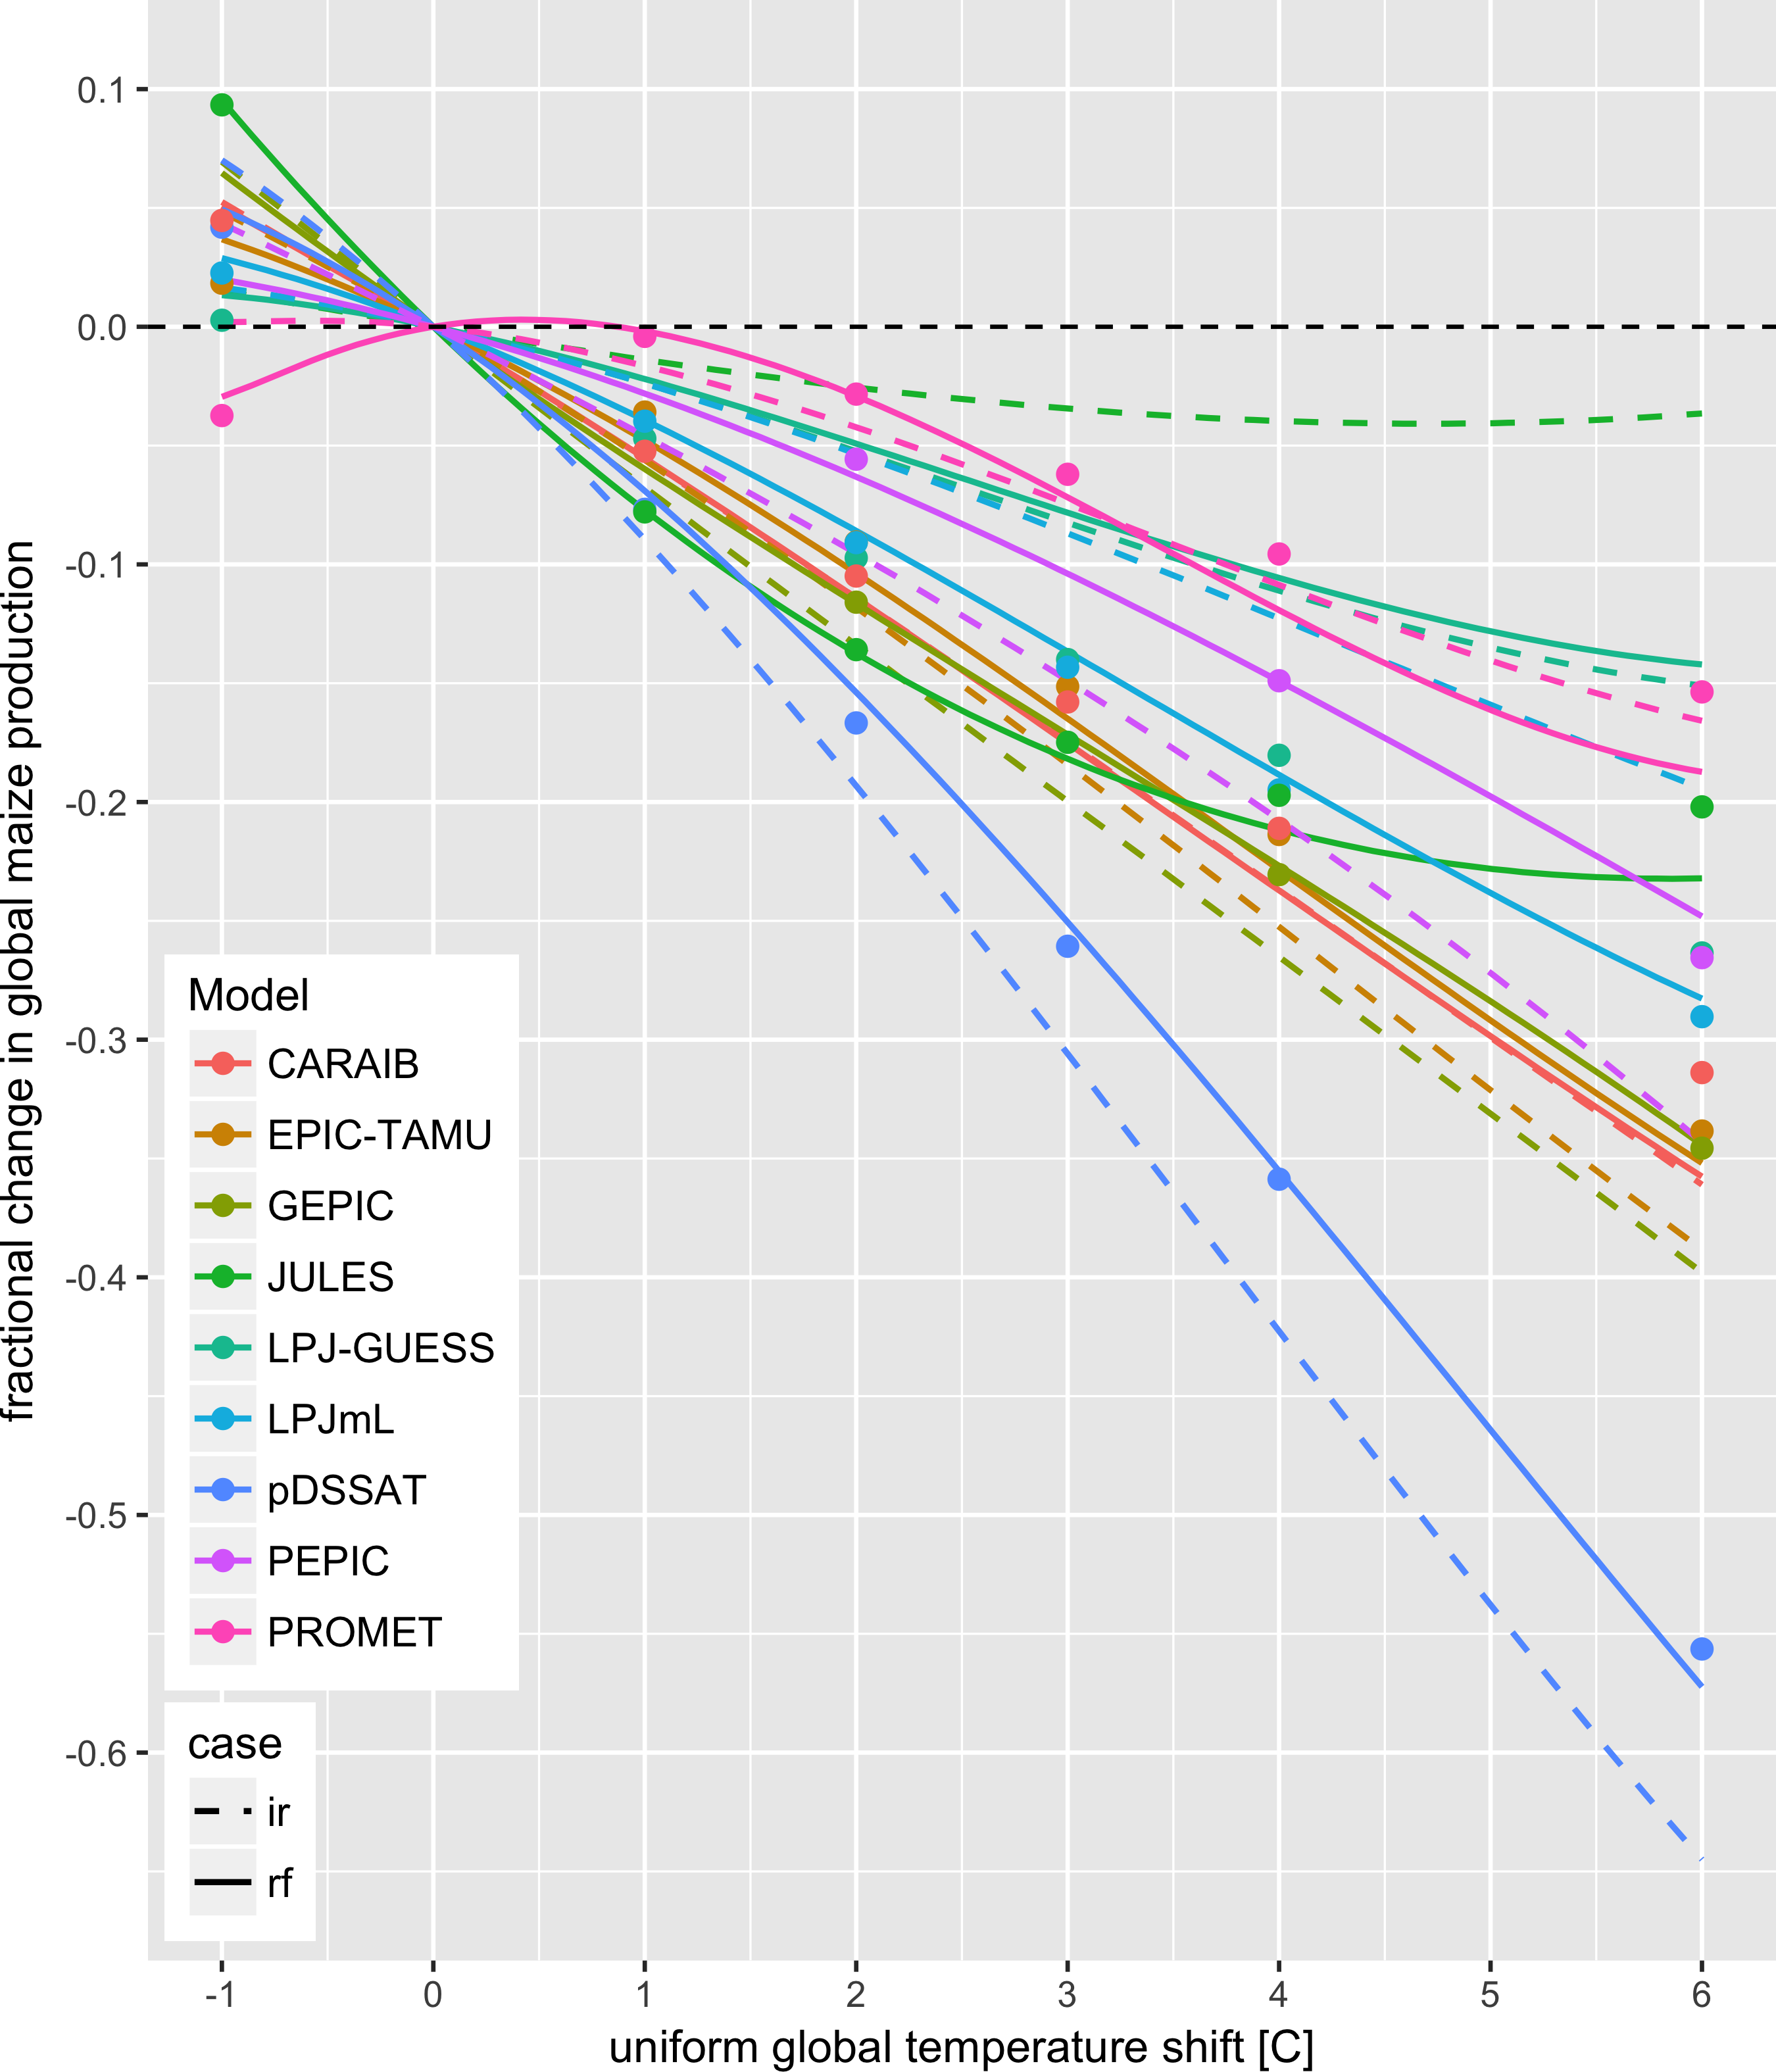
\includegraphics[width=0.95\linewidth]{figures/global_em_maize.png}
    \caption{Global emulated damages for maize on currently cultivated lands for the GGCMI Phase II models emulated, for uniform temperature shifts with other inputs held at baseline. (The damage function is created from aggregating up emulated values at the grid cell level, not from a regression of global mean yields.) Lines are emulations for rain-fed (solid) and irrigated (dashed) crops; for comparison, dots are the simulated values for the rain-fed case.  For most models, irrigated crops show a sharper reduction than do rain-fed because of the locations of cultivated areas: irrigated crops tend to be grown in warmer areas where impacts are more severe for a given temperature shift. (The exceptions are PROMET, JULES, and LPJmL.) For other crops and scenarios see Figures ~\ref{fig:temperature}- \ref{fig:nitrogen} in the supplemental material.}
    \label{fig:globe_em}
\end{figure}

\section{Conclusions and discussion} 
\label{S:6}
The GGCMI Phase II experiment provides a database targeted to allow detailed study of crop yields from process-based models under climate change. The experiment is designed to facilitate not only comparing the sensitivities of process-based crop yield models to changing climate and management inputs but also evaluating the complex interactions between driving factors (CO$_2$, temperature, precipitation, and applied nitrogen). Its global nature also allows identifying geographic shifts in high yield potential locations.  We expect that the simulations will yield multiple insights in future studies, and show here a selection of preliminary results to illustrate their potential uses. 

First, the GGCMI Phase II simulations allow identifying major areas of uncertainty. Across the major crops, inter-model uncertainty is greatest for wheat and least for soy. Across factors impacting yields, inter-model uncertainty is largest for CO$_2$ fertilization and nitrogen response effects. Across geographic regions, projections are most uncertain in the high latitudes where yields may increase, and most robust in low latitudes where yield impacts are largest.  

Second, the GGCMI Phase II simulations allow understanding the way that climate-driven changes and locations of cultivated land combine to produce yield impacts. One counterintuitive result immediate apparent is that irrigated maize shows steeper yield reductions under warming than does rain-fed maize when considered only over currently cultivated land. The effect results from geographic differences in cultivation. In any given location, irrigation increases crop resiliency to temperature increase, but irrigated maize is grown in warmer locations where the impacts of warming are more severe (Figures \ref{fig:KGirr_all}--\ref{fig:KGirr_currentcult}). The same behavior holds for rice and winter wheat, but not for soy or spring wheat (Figures \ref{fig:rice_currentcult}-\ref{fig:winter_wheat_currentcult}). Irrigated wheat and maize are also more sensitive to nitrogen fertilization levels than are analogous non-irritated crops, presumably because those rain-fed crops are limited by water as well as nitrogen availability (Figure \ref{fig:nitrogen}). (Soy as an efficient atmospheric nitrogen-fixer is relatively insensitive to nitrogen, and rice is not generally grown in water-limited conditions).

Third, we show that even the relatively limited GGCMI Phase II sampling space allows emulation of the climatological response of crop models with a relatively simple reduced-form statistical model. The systematic parameter sampling in the GGCMI Phase II procedure provides information on the influence of multiple interacting factors in a way that single projections cannot, and emulating the resulting response surface then produces a tool that can aid in both physical interpretation of the process-based models and in assessment of agricultural impacts under arbitrary climate scenarios. Emulating the climatological response isolates long-term impacts from any confounding factors that complicate year-over-year changes, and the use of simple functional forms offer the possibility of physical interpretation of parameter values. %Care should be taken in applying relationships developed at the yearly level to shifts in the mean climatology. 
We anticipate that systematic parameter sampling will become the norm in future crop model intercomparison exercises.

While the GGCMI Phase II database should offer the foundation for multiple future studies, several cautions need to be noted. Because the simulation protocol was designed to focus on change in yield under climate perturbations and not on replicating real-world yields, the models are not formally calibrated so cannot be used for impacts projections unless in used in conjunction with historical data (or data products). Because the GGCMI Phase II simulations apply uniform perturbations to historical climate inputs, they do not sample changes in higher order moments, and cannot address the additional crop yield impacts of potential changes in climate variability. Although distributional changes in model projections are fairly uncertain at present, follow-on experiments may wish to consider them. Several recent studies have described procedures for generating simulations that combine historical data with model projections of not only mean changes in temperature and precipitation but changes in their marginal distributions or temporal dependence. {\color{blue} For methods to generate adjust historical climate data inclusive of distributional and temporal dependence changes, see \citet{Leeds2015, poppick2016, Won16} and \citet{Haugen2018}). Emulation approaches are an area of active ongoing study and one of the goals of the GGCMI Phase II dataset is to facilitate these research efforts. 

%--- Probably still NEEDS EDIT --
The GGCMI Phase II output dataset invites a broad range of potential future avenues of analysis. A major target area of research is studying the models themselves including: a detailed examination of interaction terms between the major input drivers, a robust quantification of the sensitivity of different models to the input drivers, and comparisons with field-level experimental data. The parameter space tested in GGCMI Phase II will allow detailed investigations into yield variability and response to extremes under changing management and CO$_2$ levels and allow the study of geographic shifts in optimal growing regions for different crops. The output dataset also contains other runs and variables not analyzed or shown here. Runs include several which allowed adaptation to climate changes by altering growing seasons, and additional variables include above ground biomass, LAI, and root biomass (as many as 25 output variables for some models). Emulation studies that are possible include a more systematic evaluation of different statistical model specifications and formal calculation of uncertainties in derived parameters.

% -- summing up paragrah – NEEDS EDIT -- make this not sound like this paper is the end-all answer
%The future of food security is one of the larger challenges facing humanity at present. 
The development of multi-model ensembles such as GGCMI Phase II provides a way to begin to better understand crop responses to a range of potential climate inputs, improve process based models, and explore the potential benefits of adaptive responses included shifting growing season, cultivar types and cultivar geographic extent.}

%Emulation also allow making state-of-the-art simulation results available to a wide research community as simple, computationally tractable tools that can be used by downstream modelers to understand the socioeconomic impacts of crop response to climate change.   

\section{Acknowledgments}
\label{S:7}
We thank Michael Stein and Kevin Schwarzwald, who provided helpful suggestions that contributed to this work. This research was performed as part of the Center for Robust Decision-Making on Climate and Energy Policy (RDCEP) at the University of Chicago, and was supported through a variety of sources. RDCEP is funded by NSF grant \#SES-1463644 through the Decision Making Under Uncertainty program. J.F.\ was supported by the NSF NRT program, grant \#DGE-1735359. C.M.\ was supported by the MACMIT project (01LN1317A) funded through the German Federal Ministry of Education and Research (BMBF).  C.F.\ was supported by the European Research Council Synergy grant \#ERC-2013-SynG-610028 Imbalance-P. P.F. and K.W. were supported  by the Newton Fund through the Met Office Climate Science for Service Partnership Brazil (CSSP Brazil). A.S.\ was supported by the Office of Science of the U.S. Department of Energy as part of the Multi-sector Dynamics Research Program Area. Computing resources were provided by the University of Chicago Research Computing Center (RCC). S.O.\ acknowledges support from the Swedish strong research areas BECC and MERGE together with support from LUCCI (Lund University Centre for studies of Carbon Cycle and Climate Interactions).

\appendix{Simulations -- Assessment}
\label{A:1}
The GGCMI Phase II simulations are designed for evaluating changes in yield but not absolute yields, since they omit detailed calibrations.
To provide some validation of the skill of the process-based models used, we repeat the validation exercises of \citet{muller_global_2017} for GGCMI Phase I. The \citet{muller_global_2017} procedure evaluates response to year-to-year temperature and precipitation variations in a control run driven by historical climate and compares it to detrended historical yields from the FAO \citep{FAOSTAT} by calculating the Pearson correlation coefficient.  The procedure offers no means of assessing CO$_2$ fertilization, since CO$_2$ has been relatively constant over the historical data collection period. Nitrogen introduces some uncertainty into the analysis, since the GGCMI Phase II runs impose fixed, uniform nitrogen application levels that are not realistic for individual countries. % and nitrogen data are limited for many countries regardless. 
We evaluate up to three control runs for each model, since some modeling groups provide historical runs for three different nitrogen levels. %The Phase II simulations also do not reproduce realistic nitrogen application levels for individual countries, since nitrogen is one of the parameters systematically varied.

\begin{figure*}[!hb]
    \centering
    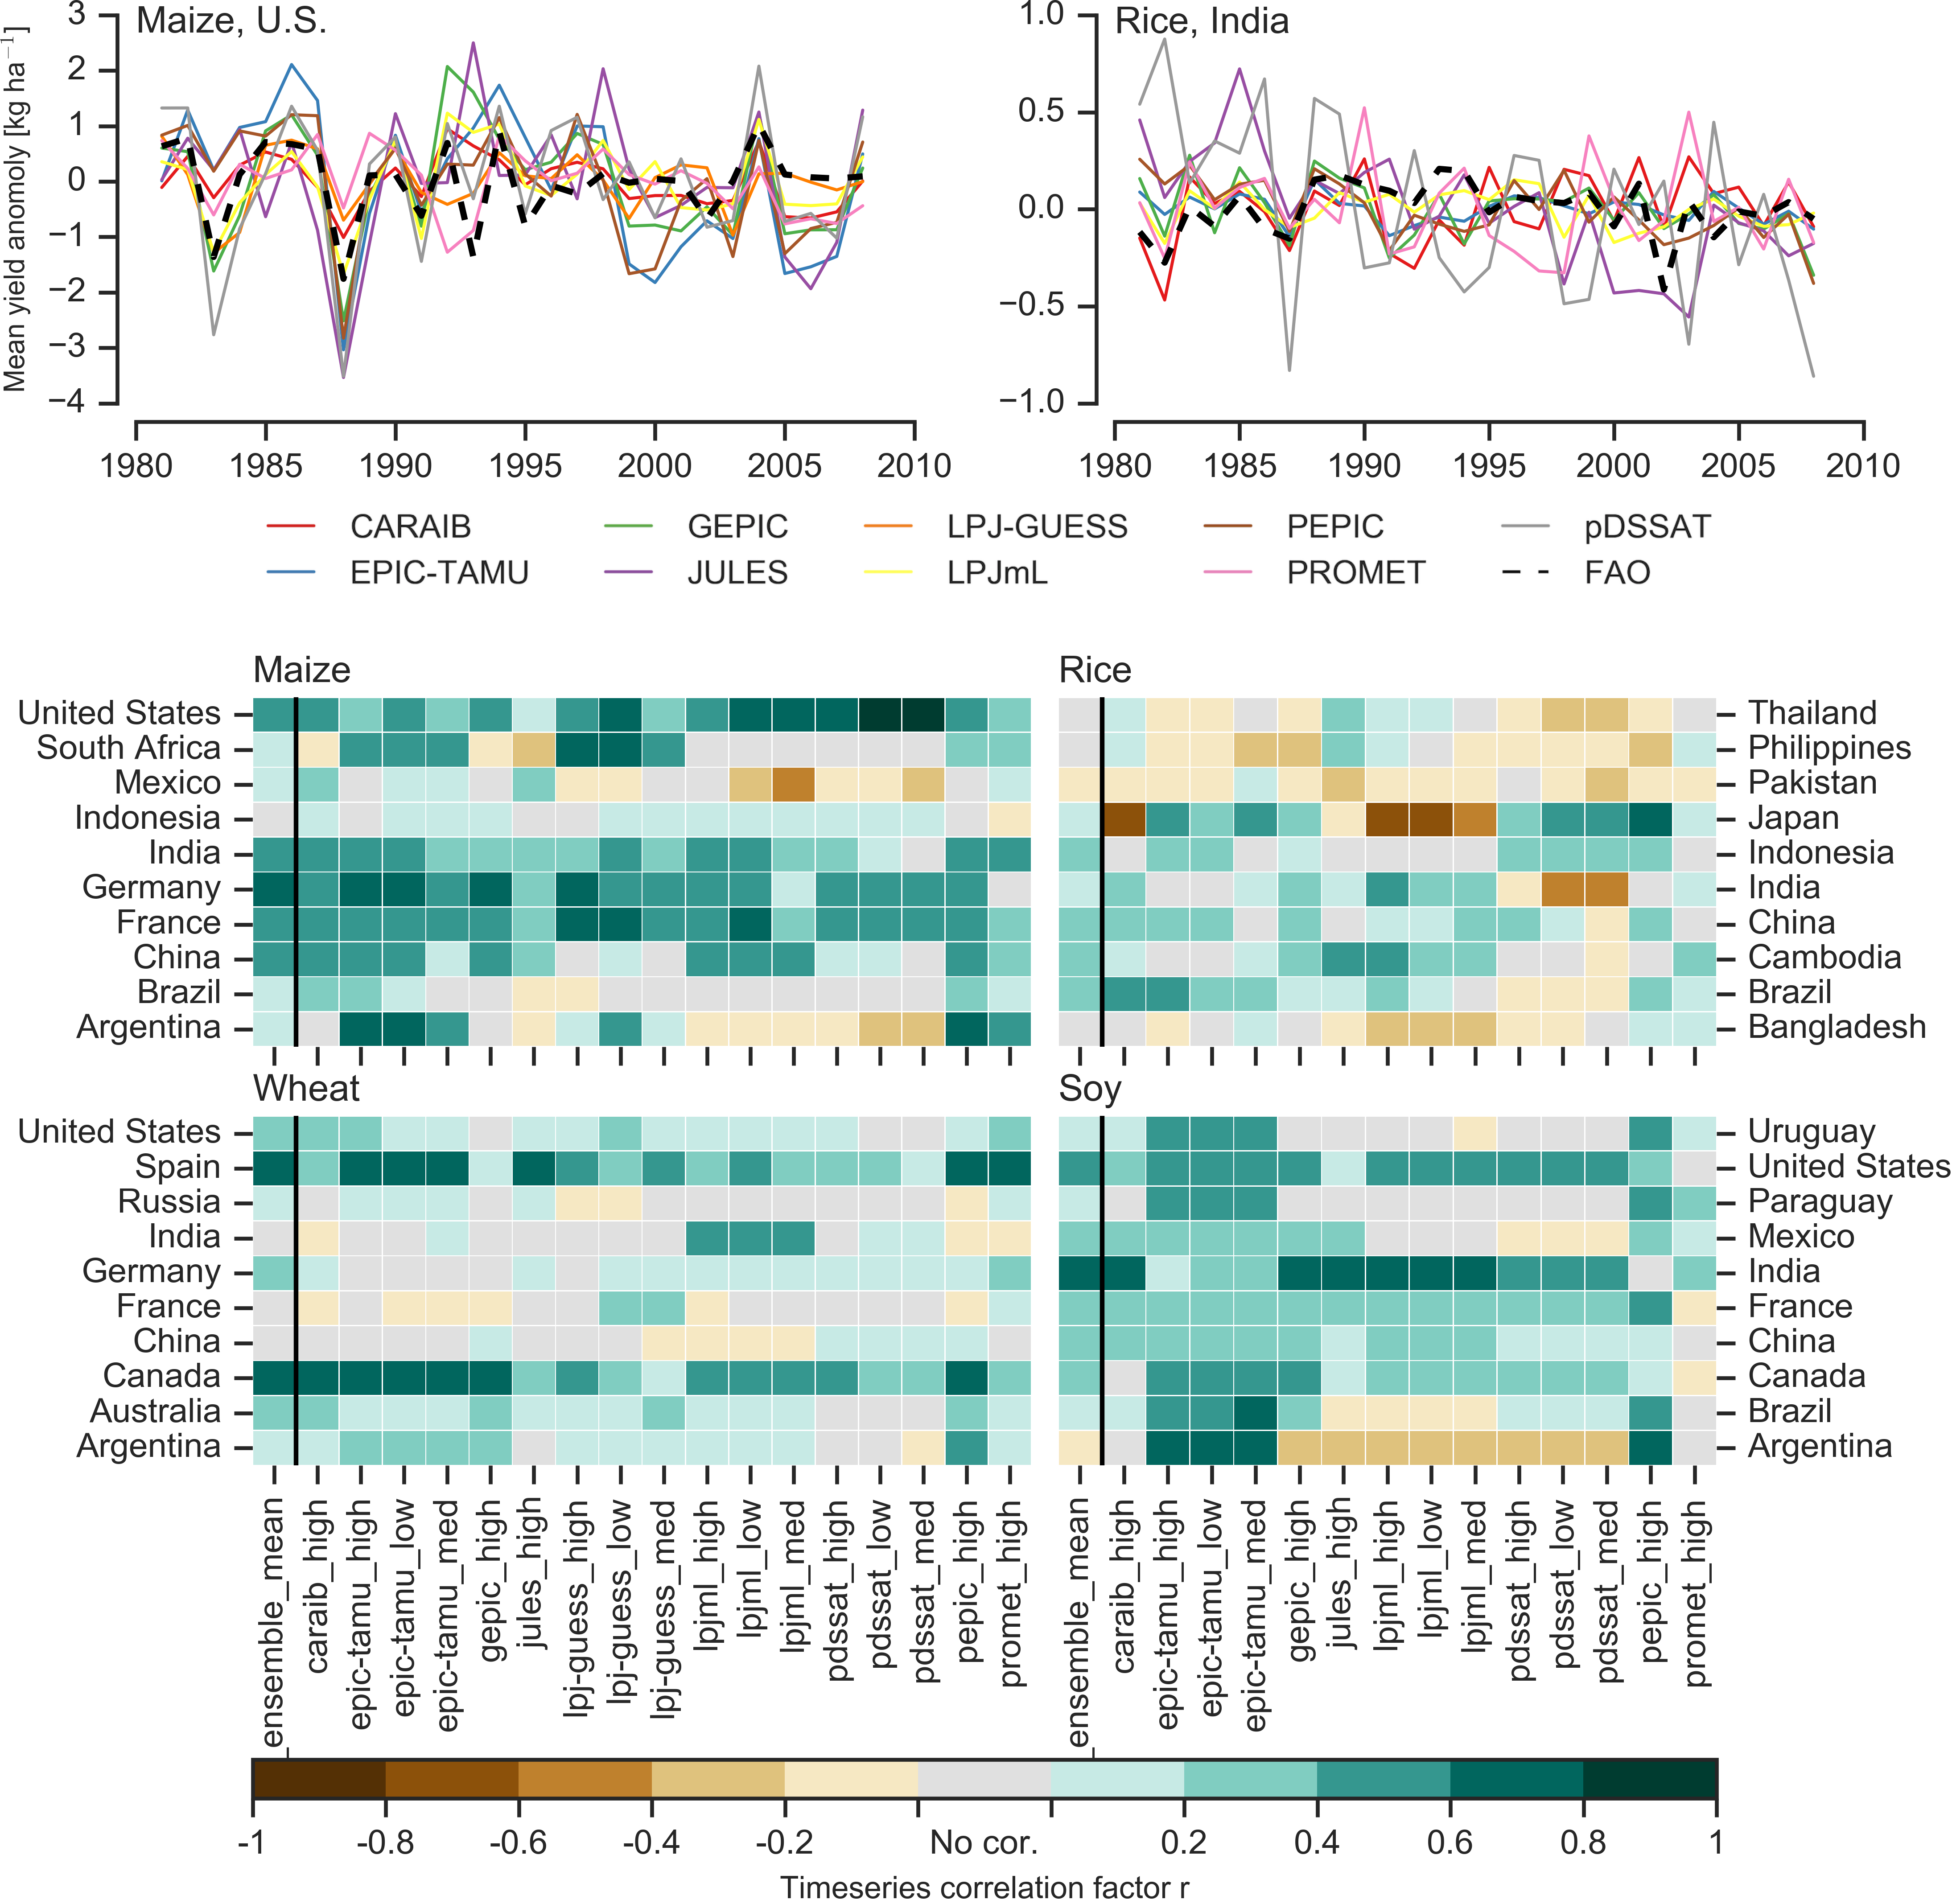
\includegraphics[width=0.95\linewidth]{figures/Agformet_validation.png}
    \caption{Time series of correlation coefficients between simulated crop yield and FAO data \citep{FAOSTAT} at the country level. The top panels indicate two example cases: US maize (a good case), and rice in India (mixed case), both for the high nitrogen application case. The heatmaps illustrate the Pearson $r$ correlation coefficient between the detrended simulation mean yield at the country level compared to the detrended FAO yield data for the top producing countries for each crop with continuous FAO data over the 1980-2010 period. Models that provided different nitrogen application levels are shown with low, med, and high label (models that did not simulated different nitrogen levels are analogous to a high nitrogen application level). The ensemble mean yield is also correlated with the FAO data (not the mean of the correlations). Wheat contains both spring wheat and winter wheat simulations.}
    \label{fig:simulation_val}
\end{figure*}

{\color{blue} Figure \ref{fig:simulation_val} shows the Pearson time series correlation between the simulation model yield and FOA yield data. Figure \ref{fig:simulation_val} can be compared to Figures 1,2,3,4 and 6 in \citet{muller_global_2017}. The results are mixed, with many regions for rice and wheat being difficult to model. No single model is dominant, with each model providing near best-in-class performance in at least one location-crop combination. The presence of very few vertical dark green color bars clearly illustrates the power of a multi-model intercomparison project like the one presented here. The ensemble mean does not beat the best model in each case, but shows positive correlation in over 75\% of the cases presented here. The EPIC-TAMU model performs best for soy, CARIAB, EPIC-TAMU, and PEPIC perform best for maize, PROMET performs best for wheat, and the EPIC family of models perform best for rice. Reductions in skill over the performance illustrated in \citet{muller_global_2017} may be attributed to the nitrogen levels or lack of calibration in some models.

%Soy is qualitatively the easiest crop to represent (except in Argentina), which is likely due in part to the invariance of the response to nitrogen application (soy fixes atmospheric nitrogen very efficiently). Comparison to the FAO data is therefore easier than the other crops because the nitrogen application levels do not matter. US maize has the best performance across models, with nearly every model representing the historical variability to a reasonable extent. Especially good example years for US maize are 1983, 1988, and 2004 (top left panel of Figure \ref{fig:simulation_val}), where every model gets the direction of the anomaly compared to surrounding years correct. 1983 and 1988 are famously bad years for US maize along with 2012 (not shown). US maize is possibly both the most uniformly industrialized (in terms of management practices) crop and the one with the best data collection in the historical period of all the cases presented here.

The FAO data is at least one level of abstraction from ground truth in many cases, especially in developing countries. The failure of models to represent the year-to-year variability in rice in some countries in southeast Asia is likely partly due to model failure and partly due to lack of data. It is possible to speculate that the difference in performance between Pakistan (no successful models) and India (many successful models) for rice may reside at least in part in the FAO data and not the models themselves. The same might apply to Bangladesh and India for rice. %Partitioning of these contributions is impossible at this stage. 
Additionally, there is less year-to-year variability in rice yields (partially due to the fraction of irrigated cultivation). Since the Pearson r metric is scale invariant, it will tend to score the rice models more poorly than maize and soy. 
%An example of very poor performance can be seen with the pDSSAT model for rice in India (top right panel of Figure \ref{fig:simulation_val}).}

\begin{figure}[!p]
\centering
    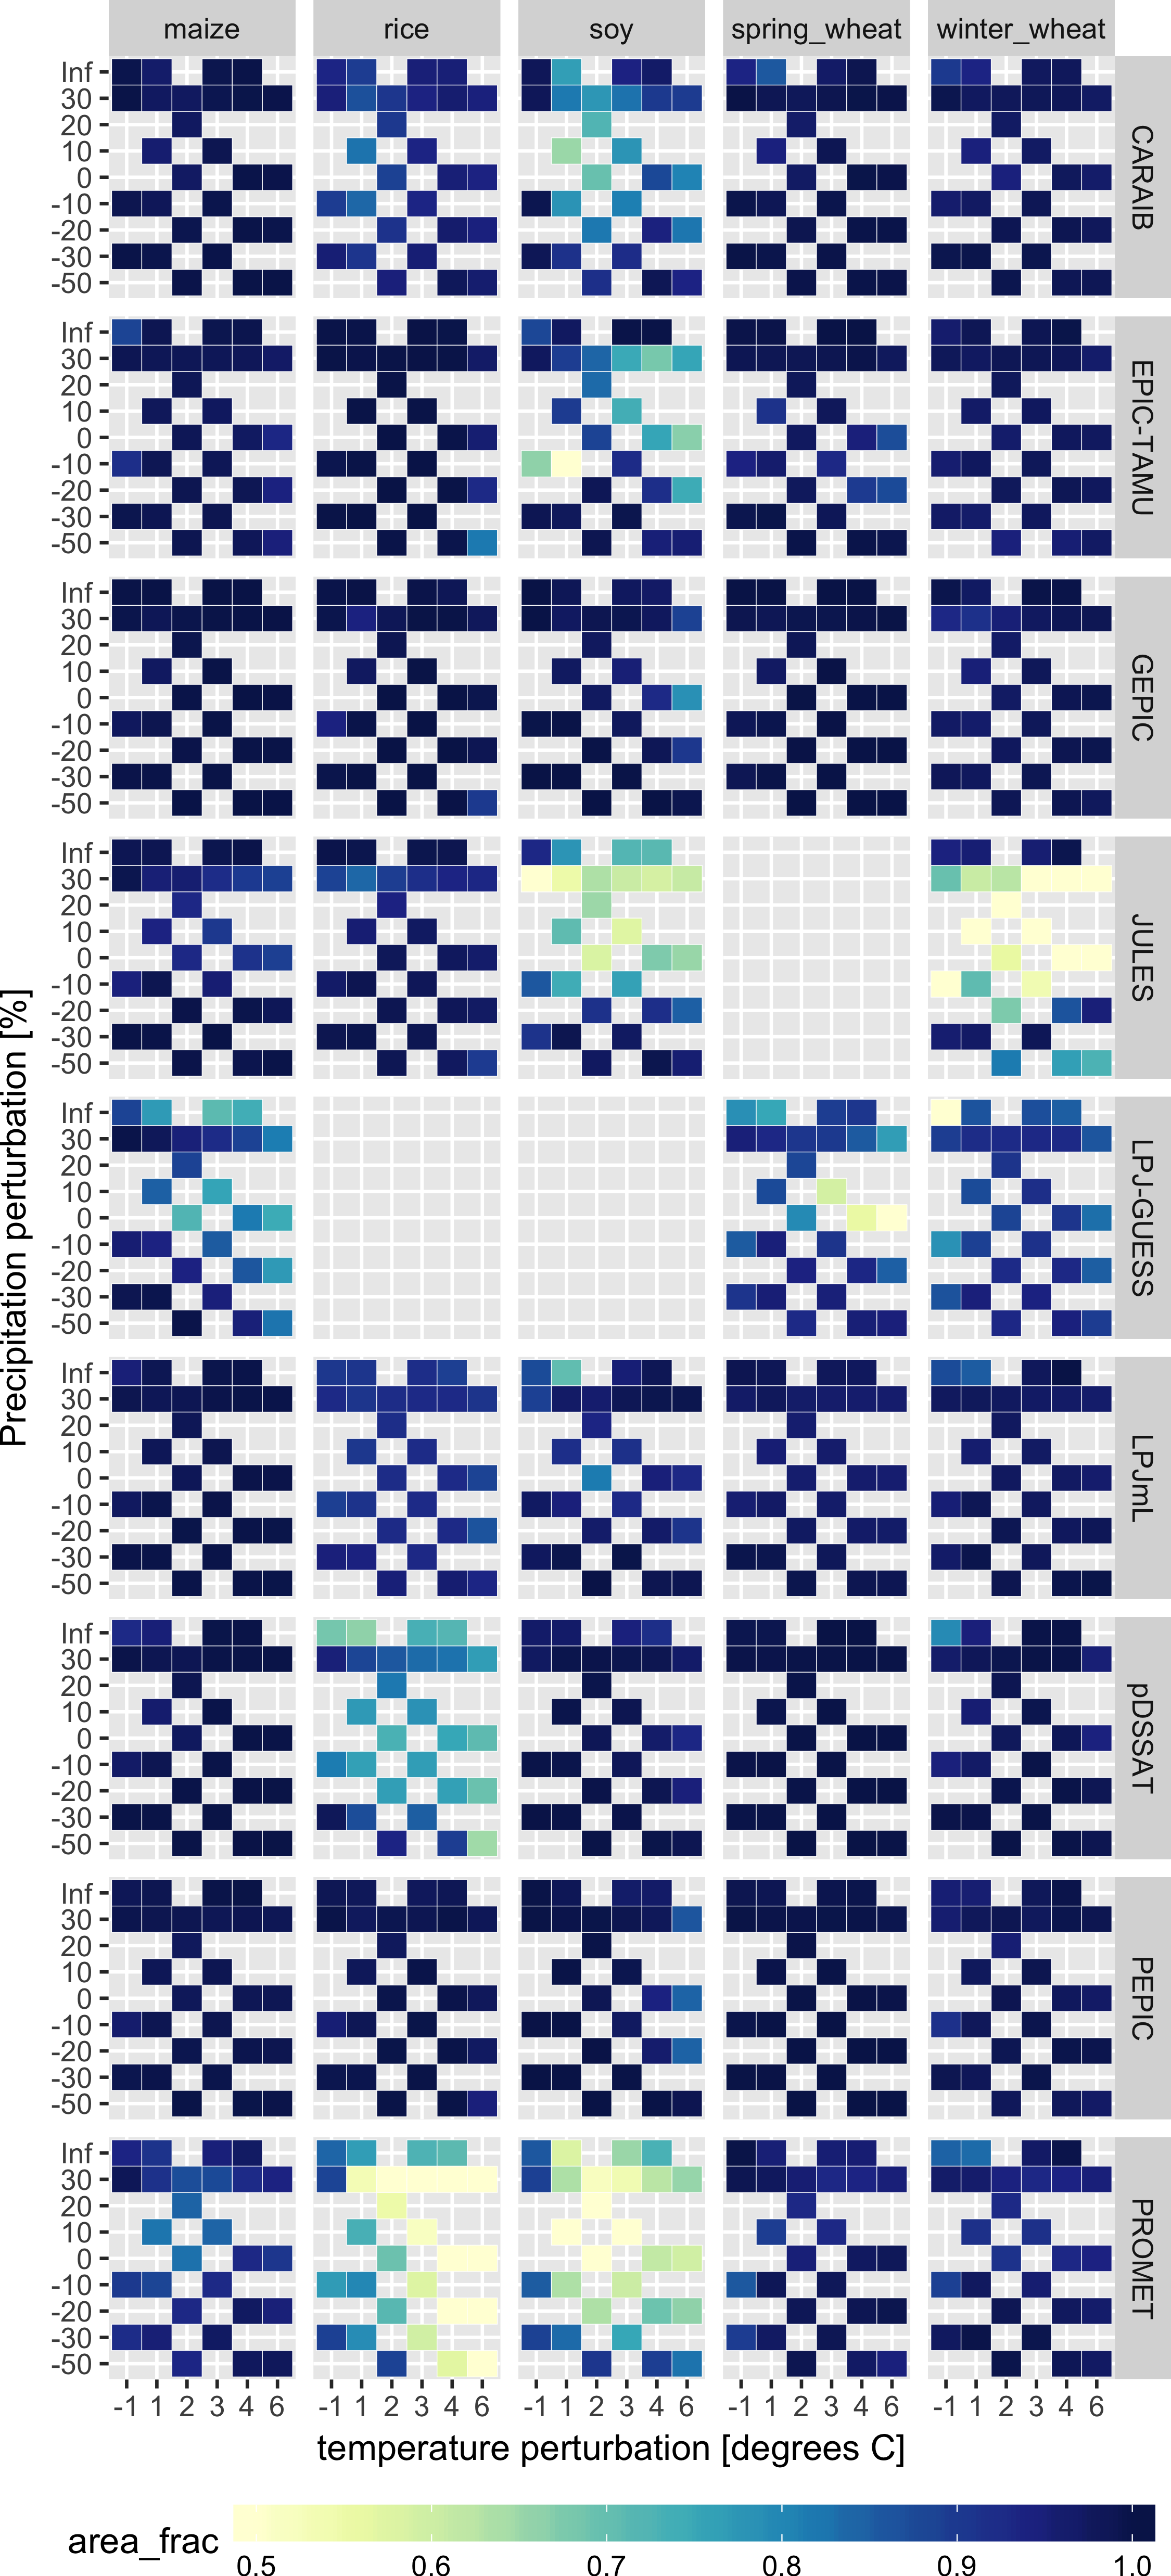
\includegraphics[width=1\linewidth]{figures/error_360.png}
    \caption{Assessment of emulator performance over currently cultivated areas based on normalized error (Equations \ref{eqn:error}, \ref{eqn:per_yield}). We show performance of all 9 models emulated, over all crops and all sampled T and P inputs, but with CO$_2$ and nitrogen held fixed at baseline values. Large columns are crops and large rows models; squares within are T,P scenario pairs. Colors denote the fraction of currently cultivated hectares ('area_frac') for each crop with normalized area $e$ less that 1 indicating the the error between the emulation and simulation less that one standard deviation of the ensemble simulation spread. Of the 756 scenarios with these CO$_2$ and N values, we consider only those for which all 9 models submitted data. JULES did not simulate spring wheat and LPJ-GUESS did not simulate rice and soy. Emulator performance is generally satisfactory, with some exceptions. Emulator failures (significant areas of poor performance) occur for individual crop-model combinations, with performance generally degrading for hotter and wetter scenarios.}
   \label{fig:error_360}
\end{figure}

\begin{figure}[!p]
\centering
    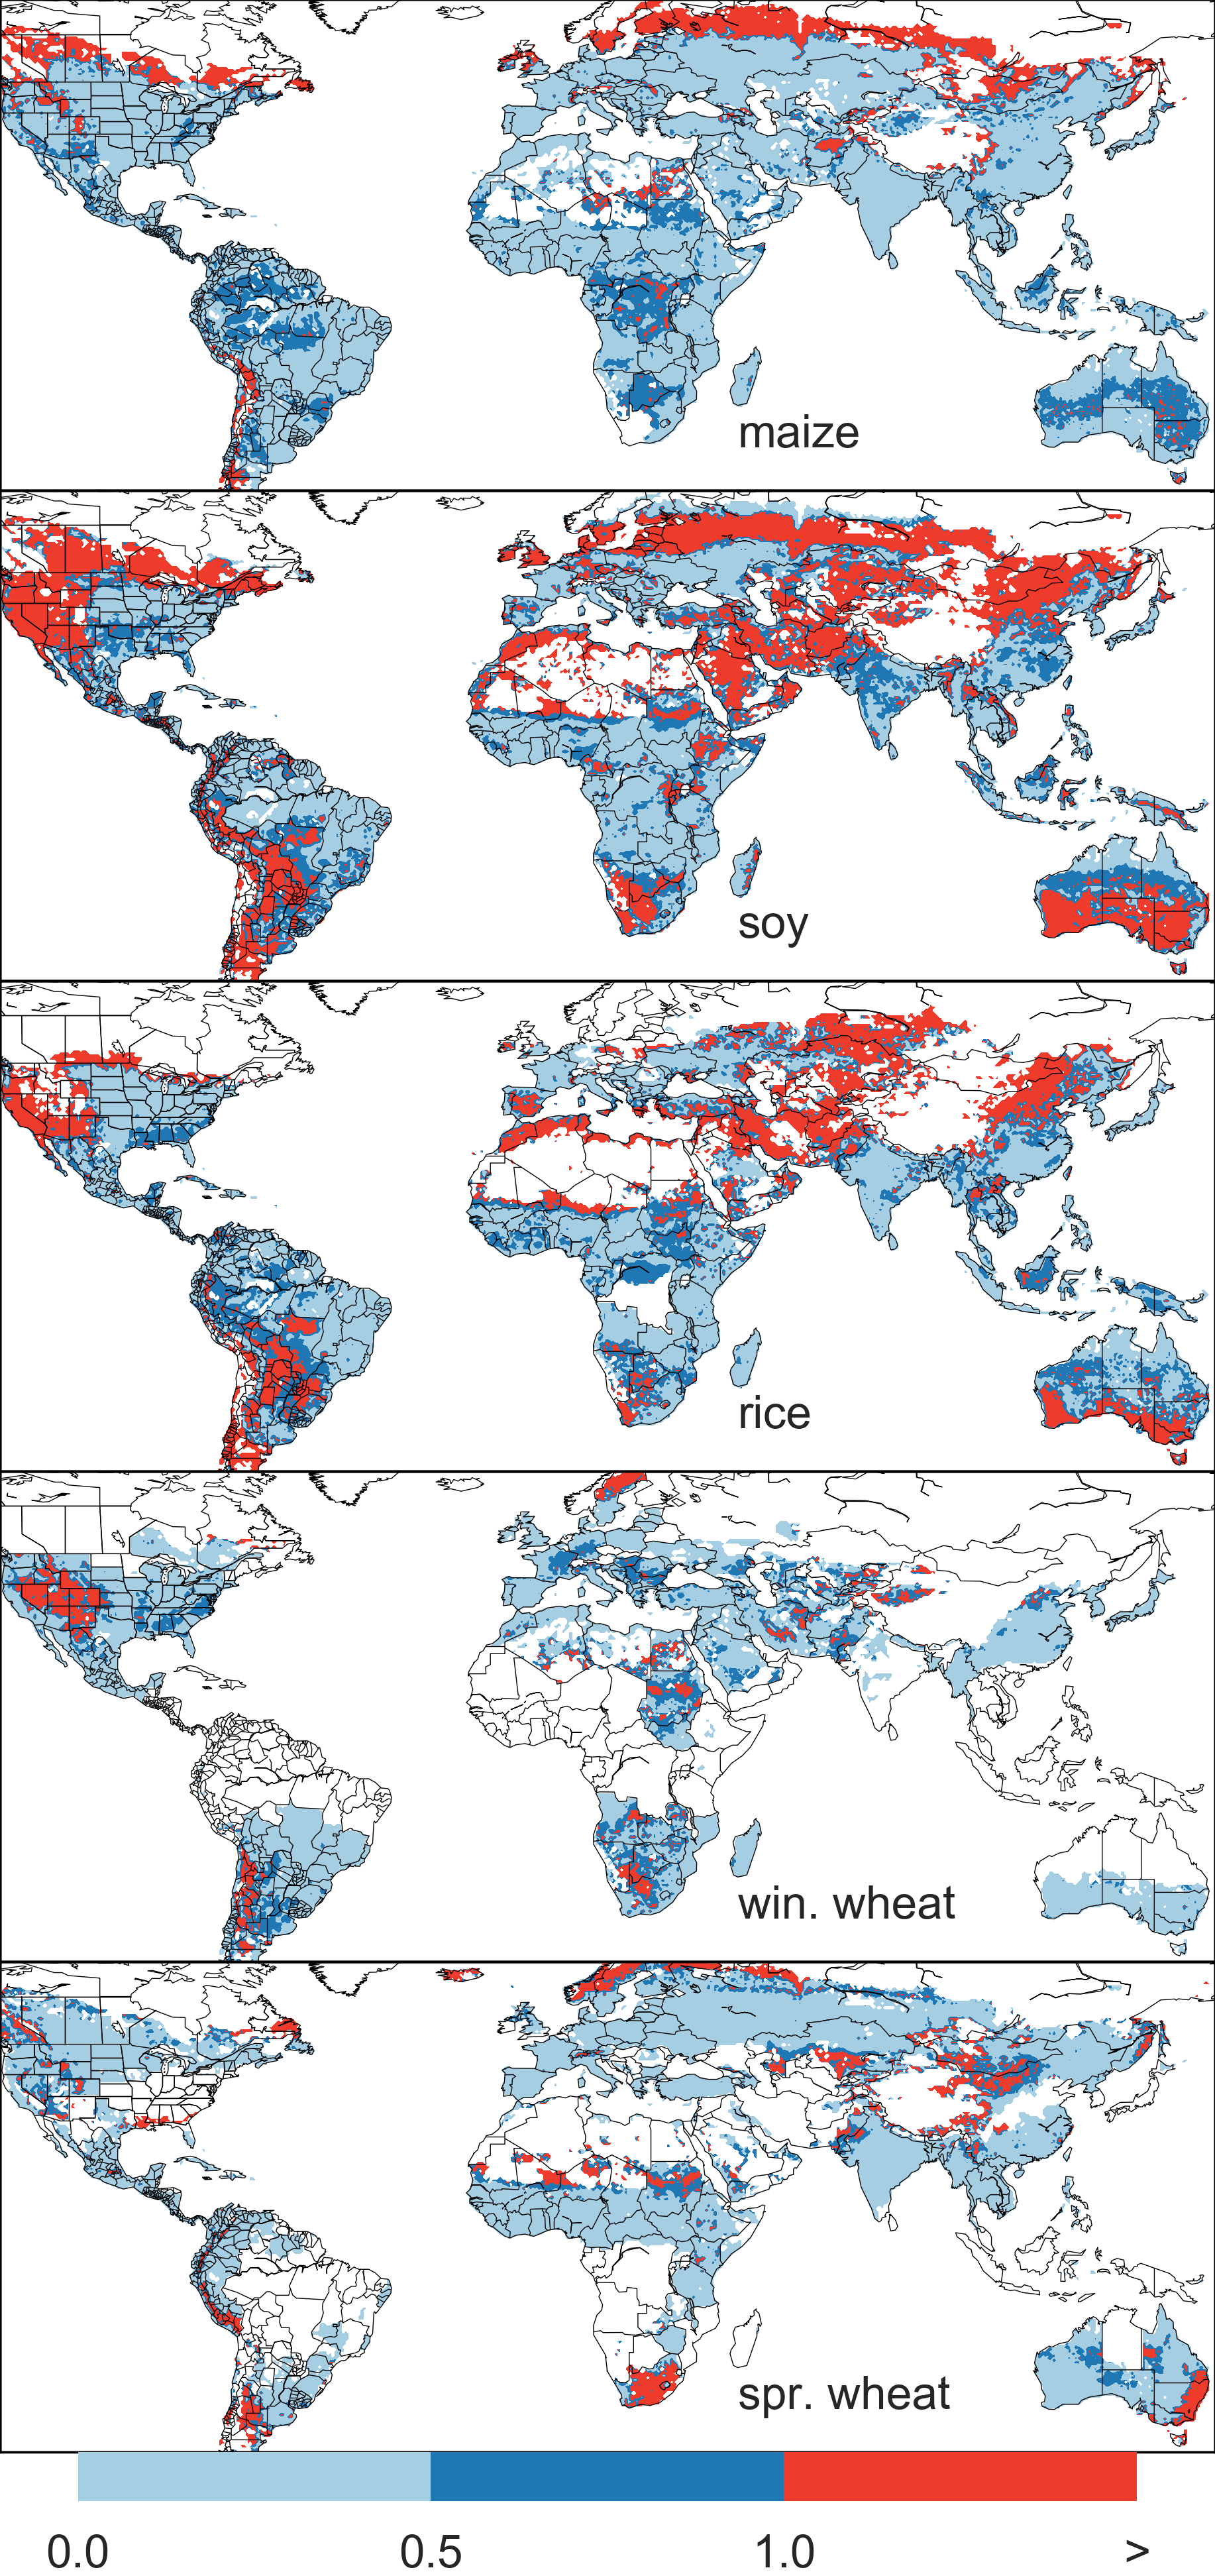
\includegraphics[width=0.95\linewidth]{figures/em_err.png}
    \caption{Illustration of our test of emulator performance, applied to the CARAIB model for the T+4 scenario for rain-fed crops. Contour colors indicate the normalized emulator error $e$, where $e > 1$ means that emulator error exceeds the multi-model standard deviation. White areas are those where crops are not simulated by this model. Models differ in their areas omitted, meaning the number of samples used to calculate the multi-model standard deviation is not spatially consistent in all locations. Emulator performance is generally good relative to model spread in areas where crops are currently cultivated (compare to Figure 1) and in temperate zones in general; emulation issues occur primarily in marginal areas with low yield potentials. For CARAIB, emulation of soy is more problematic, as was also shown in Figure \ref{fig:error_360}.}
   \label{fig:error}
\end{figure}

\appendix{Emulation -- Assessment}
\label{A:2}

Because no general criteria exist for defining an acceptable crop model emulator, we utilize a metric of emulator performance specific to GGCMI Phase II. For a multi-model comparison exercise like GGCMI Phase II, one reasonable criterion is what we term the ``normalized error'', which compares the fidelity of an emulator for a given model and scenario to the inter-model uncertainty. We define the normalized error $e$ for each scenario as the difference between the fractional yield change from the emulator and that in the original simulation, divided by the standard deviation of the multi-model spread (Equations \ref{eqn:per_yield} and  \ref{eqn:error}):

\begin{equation}
    \label{eqn:per_yield}
    F_{\: scn.}=\frac{Y_{scn.}-Y_{baseline}}{Y_{baseline}}
\end{equation}

\begin{equation}
    \label{eqn:error}
    e_{\: scn.} =\frac{F_{em, \: scn.}-F_{sim, \: scn.}}{\sigma_{sim, \: scn.}}
\end{equation}

Here $F_{\: scn.}$ is the fractional change in a model's mean emulated or simulated yield from a defined baseline, in some scenario (scn.) in C, T, W, and N space; $Y_{scn.}$ and $Y_{baseline}$ are the absolute emulated or simulated mean yields. The normalized error $e$ is the difference between the emulated fractional change in yield and that actually simulated, normalized by $\sigma_{sim}$, the standard deviation in simulated fractional yields $F_{sim,\: scn.}$ across all models. The emulator is fit across all available simulation outputs, and then the error is calculated across the simulation scenarios provided by all nine models (Figure \ref{fig:error_360} and Figures \ref{fig:error360total} and Figures \ref{fig:error810} in supplemental documents). 

To assess the ability of the polynomial emulation to capture the behavior of complex process-based models, we evaluate the normalized emulator error. That is, for each grid cell, model, and scenario we evaluate the difference between the model yield and its emulation, normalized by the inter-model standard deviation in yield projections. This metric implies that emulation is generally satisfactory, with several distinct exceptions. Almost all model-crop combination emulators have normalized errors less than one over nearly all currently cultivated hectares (Figure \ref{fig:error_360}), but some individual model-crop combinations are problematic (e.g.\ PROMET for rice and soy, JULES for soy and winter wheat, Figures \ref{fig:errorjules}--\ref{fig:errorpromet}). Normalized errors for soy are somewhat higher across all models not because emulator fidelity is worse but because models agree more closely on yield changes for soy than for other crops (see Figure \ref{fig:temperature}, lowering the denominator. Emulator performance often degrades in geographic locations where crops are not currently cultivated. Figure \ref{fig:error} shows a CARAIB case as an example, where emulator performance is satisfactory over cultivated areas for all crops other than soy, but uncultivated regions show some problematic areas. 

Note that the normalized error $e$ for a model depends not only on the fidelity of its emulator in reproducing a given simulation but on the particular suite of models considered in the intercomparison exercise. The rationale for this choice is to relate the fidelity of the emulation to an estimate of true uncertainty, which we take as the multi-model spread. 
{\color{red} Because the inter-model spread is large, normalized errors tend to be small. That is, any failures of emulation are small relative to inter-model uncertainty. We therefore do not provide a formal parameter uncertainty analysis, but note that the GGCMI Phase II dataset is well-suited to statistical exploration of emulation approaches and quantification of emulator fidelity.} %, including exercises such as withholding some simulations from the training set and evaluating the ability of the resulting emulator to reproduce the ``test'' scenarios.}  

It should be noted that this assessment metric is relatively forgiving. First, each emulation is evaluated against the simulation actually used to train the emulator. Had we used a spline interpolation the error would necessarily be zero. Second, the performance metric scales emulator fidelity not by the magnitude of yield changes but by the inter-model spread in those changes. Where models differ more widely, the standard for emulators becomes less stringent. Because models disagree on the magnitude of CO$_2$ fertilization, this effect is readily seen when comparing assessments of emulator performance in simulations at  baseline CO$_2$ (Figure \ref{fig:error_360}) with those at higher CO$_2$ levels (Figure \ref{fig:error810}). Widening the inter-model spread leads to an apparent increase in emulator skill.

\section{References}
\label{S:6}

%% \appendix
%% \section{}
%% \label{}

%% References
%% Following citation commands can be used in the body text:
%% Usage of \cite is as follows:
%%   \cite{key}          ==>>  [#]
%%   \cite[chap. 2]{key} ==>>  [#, chap. 2]
%%   \citet{key}         ==>>  Author [#]
\bibliography{bib.bib}

%\printbibliography
%% References with bibTeX database:
%% Authors are advised to submit their bibtex database files. They are requested to list a bibtex style file in the manuscript if they do not want to use model1-num-names.bst.

\end{document}
%% End of file `elsarticle-template-1-num.tex'.

%%%%%%%%%%%%%%%%%%%%%%%%%%%%%%%%%%%%%%%%%%%%%%%%%%%%%%%%%%%%%%%%
%%%%%%%%%%%%%%%%%%%%%%%%%%%%%%%%%%%%%%%%%%%%%%%%%%%%%%%%%%%%%%%%
%%%%%%%%%%%%%%%%%%%%%%%%%%%%%%%%%%%%%%%%%%%%%%%%%%%%%%%%%%%%%%%%
%%%%%%%%%%%%%%%%%%%%%%%%%%%%%%%%%%%%%%%%%%%%%%%%%%%%%%%%%%%%%%%%
% notes from Liz

%there are a lot of results in Conclusions/Discussion, some of which are only thinly discussed - might get asked to move them or justify more. (Unless you moved these already)

%- why not compare your emulator to statistical models from others?  You might say because models weren't calibrated, but it's a reasonable and may have to be addressed.

%- if we didn't state the irrigated/unirrigated conclusion in the abstract, we should do that

%- on irrigated/unirrigated figures in supp docs - for the currently cultivated land, put the mean temp for the relevant area for irrigated and unirrigated, to back up assertion in paper that there is a temperature difference.

%- We claimed that irrigated damages were higher because damages for a given T change are larger for a given baseline temperature. Is that backed up in the paper? Only indirectly by the maps that show stronger damages in the T+4 case for low latitudes than high latitudes. It could be interesting to do scatterplot of yield changes for a given scenario where the x axis is baseline climate. (Or include two scenarios colored differently...)

%- probably good to explain in more detail that simpler fitting methods can cause problems. Even just a sentence or two in the main manuscript to explain that your choice is better. If you wanted to put in the results of more methodological work, that could work too, either in the main paper or the supp docs. Part of the paper's message is that emulation is possible; it would make sense to explain that it is NOT possible to emulate well if you don't use the right approach.

%%%%%%%%%%%%%%%%%%%%%%%%%%%%%%%%%%%%%%%%%%%%%%%%%%%%%%%%%%%%%%%%
%%%%%%%%%%%%%%%%%%%%%%%%%%%%%%%%%%%%%%%%%%%%%%%%%%%%%%%%%%%%%%%%
%%%%%%%%%%%%%%%%%%%%%%%%%%%%%%%%%%%%%%%%%%%%%%%%%%%%%%%%%%%%%%%%
%%%%%%%%%%%%%%%%%%%%%%%%%%%%%%%%%%%%%%%%%%%%%%%%%%%%%%%%%%%%%%%%
